\documentclass[a4paper,11pt]{scrreprt}

\usepackage[utf8]{inputenc}
\usepackage[ngerman]{babel}
\usepackage[T1]{fontenc}
\usepackage{amsmath}
\usepackage{graphicx}
\usepackage{xcolor}
\usepackage{wrapfig}
\usepackage{multirow}
\usepackage{ulem}
\usepackage{booktabs}
\usepackage{caption}
\usepackage{subcaption}
\usepackage{url}
\usepackage{fancyhdr}
\usepackage{lscape}
\usepackage{hyperref}
\usepackage{blindtext}
\usepackage{adjustbox}
\usepackage[top=3.5cm,bottom=3.5cm,left=2.5cm,right=2.5cm]{geometry}

\bibliographystyle{unsrt}
\parindent0pt

%Kopf-& Fusszeile----------------------------
\pagestyle{fancy}
\lhead{
\includegraphics[width=1.5cm]{Bilder/fhnw_logo.png}}
\chead{Elektro- und Informationstechnik}
\renewcommand{\headrulewidth}{0.4pt}
%--------------------------------------------

\renewcommand*\chapterheadstartvskip{\vspace*{-0.2cm}}

\begin{document}
\thispagestyle{empty}

\begin{center}
\begin{tabular}{p{\textwidth}}

\begin{flushleft}

\includegraphics[scale=1.3]{Bilder/FHNW.png}
\end{flushleft}

\\

\\

\begin{center}
\textcolor{black}{
\textbf{
\Huge{
Fachbericht
}}}
\end{center}

\\

\begin{center}
\Large{
\textbf{
Projekt 4
}}
\end{center}

\\

\begin{center}
\large{
Fachhochschule Nordwestschweiz FHNW
}
\end{center}

\\

\begin{center}
\large{\today}
\end{center}

\vspace*{2cm}

\begin{center}
\begin{tabular}{ll}
\toprule 
\textbf{Studiengang:} 		& Elektro- und Informationstechnik EIT \\
\hline
\textbf{Auftraggeber/in:} 	& Prof. Hans Gysin\\
							& Jana Kalbermatter\\
\hline
\textbf{Fachexperten:} 		& Matthias Meier \\
							& Prof. Dr. Pascal Schleuniger \\
							& Pascal Buchschacher \\
							& Dr. Roswitha Dubach \\
							& Dr. Anita Gertiser \\
							& Bonnie Domenghino \\
\hline
\textbf{Projektteam:} & Adrian Annaheim \\ 
							& Benjamin Ebeling \\ 
 							& Jonas Rosenmund\\ 
 							& Michael Schwarz  \\ 
 							& Samuel Wey \\ 
 							& Andres Minder \\ 
\bottomrule
\end{tabular}
\end{center}

\end{tabular}
\end{center}

\tableofcontents \thispagestyle{fancy}  \cfoot{} \renewcommand{\footrulewidth}{0pt} \rhead{\slshape Inhaltsverzeichnis}

% ab hier ist diese Konvention für die Fusszeile eingestellt
\lfoot{Team 1\\Projekt 4}
\cfoot{\thepage}
\rfoot{\today}
\renewcommand{\footrulewidth}{0.4pt}

\chapter{Einleitung}
% ================ Einstellungen =======================
\thispagestyle{fancy} \rhead{\slshape Einleitung} \setcounter{page}{1}
% ======================================================
Museen haben die Aufgabe, mit Ausstellungen spezifische Themenbereiche den Interessierten zugänglich und erlebbar zu machen. Dabei soll oft ein breites Publikum vom wenig Informierten bis zur Expertin angesprochen werden. Um den Besuchenden zu ermöglichen, sich mit den persönlich relevanten Objekten auseinanderzusetzen, werden unter anderem Audioguides verwendet. Diese Audioguides werden meist zusammen mit Standard-Kopfhörern eingesetzt. Um den Hygienestandards zu entsprechen, müssen die Kopfhörer entweder aufwändig gereinigt oder Einwegkopfhörer eingesetzt werden. Der Kostenaufwand ist verhältnismässig gross, zudem bieten die bisher verwendeten Audioguides keine Möglichkeit, eine Ausstellung aufzuteilen. Eine Unterteilung der Ausstellung würde den Museen neue Angebote ermöglichen, z. B. Eintrittskarten für ausgewählte Ausstellungsbereiche mit entsprechend individualisierten Audioguides anzubieten. Dies könnte eine Museumsausstellung attraktiver gestalten. \\

Ziel dieser Projektarbeit war es, einen Audioguide namens Dojo mit der notwendigen Elektronik auszustatten. Das Konzept Dojo wurde bereits erarbeitet, das heisst im Rahmen dieser Arbeit stand die technische Umsetzung des Konzeptes von Dojo im Zentrum. Dojo soll eine Ausstellung eingrenzen können, indem es nur die gewählten Audiodateien abspielt und allenfalls als Zutrittsberechtigung fungiert.  Die Audioübertragung vom Gerät ans Gehör soll über einen Knochenschallgeber realisiert werden, um die Unterhaltskosten der Geräte signifikant zu senken. Mit Hilfe des Audioguides soll es möglich sein, Sounddateien abzuspielen, sobald man sich in der Nähe eines Ausstellungsobjektes befindet. Dojo soll zudem eine Funktion, welche einem Like-Button ähnlich ist, besitzen. Diese Funktion soll dem Besucher und der Besucherin ermöglichen, Objekte auszuwählen und später mehr Informationen darüber z. B. in Form einer Broschüre zu erhalten. Die zu entwickelnde Elektronik muss in dem bereits bestehenden Design Platz finden. \\

Um die gewünschten Audiodateien freizuschalten und den richtigen Ausstellungsobjekten zuzuordnen, wird am Anfang des Besuches ein Schlüssel auf das Dojo geladen, welcher anhand einer Korrespondenztabelle die ausgewählten Dateien freischaltet. Mit Hilfe von Bluetooth-Beacons, welche im Museum bei den Objekten befestigt sind, können den Ausstellungsobjekten Audiodateien zugeordnet werden. Durch einen Vibrationsmotor wird signalisiert, dass eine Audiodatei abspielbereit ist. Die Audiodatei, welche sich auf einer $\mu$SD-Karte befindet, wird nach Betätigung des Start-Buttons über einen WTV020 Chip auf dem Knochenschallgeber abgespielt. Wenn der Like-Button während dem Rundgang betätigt wird, kann anschliessend am Ausgang über die Korrespondenztabelle eine individuelle Broschüre ausgedruckt werden oder man kann sich die Broschüre als PDF per E-Mail zusenden lassen.\\

Mit Hilfe des hergestellten Prototyps ist es möglich, Beacons in einem Abstand von xxx Metern korrekt zu erfassen und die zugeordnete Audiodatei abzuspielen. Auf dem Dojo können maximal 512 Audiodateien abgespeichert werden. Am Eintritt können je nach Wunsch die verschiedenen Audiofiles ausgewählt werden und für den Besuch freigegeben werden. Den Besuchern und den Besucherinnen wird die Möglichkeit gegeben, für gewünschte Objekte mit Hilfe eines Like-Buttons am Ende des Museumsrundgangs Zusatzinformationen in Form einer Broschüre zu erhalten.\\
 
In dem nachfolgenden Kapitel Grundkonzept, wird die Aufteilung des Berichtes dargelegt. 


\chapter{Gesamtsystem}
% ================ Einstellungen =======================
\thispagestyle{fancy} \rhead{\slshape Gesamtsystem}
% ======================================================



\definecolor{myviolett}{RGB}{212,192,226}
\definecolor{myyellow}{RGB}{255,255,178}
\definecolor{myorange}{RGB}{252,231,218}
\definecolor{mygreen}{RGB}{229,241,221}
\definecolor{myblue}{RGB}{225,237,247}
\definecolor{myred}{RGB}{255,178,178}


Abbildung \ref{Blockschaltbild_Gesamtsystem} zeigt das grobe Gesamtsystem des Dojos. Die einzelnen Kapitel dieses Berichts orientieren sich an den Blöcken und deren Funktion im Gesamtsystem. In Kapitel \textbf{\ref{Software} \nameref{Software}} wird die Computersoftware erklärt, welche verwendet wird, um das Dojo zu konfigurieren. Das Kapitel \textbf{\ref{Energieversorgung} \nameref{Energieversorgung}} befasst sich mit dem Akku, der Ladeschaltung und -überwachung, sowie der Spannungsversorgung. Im Kapitel \textbf{\ref{USB} \nameref{USB}} wird erläutert, wie über die USB-Schnittstelle mit dem Mikrocontroller kommuniziert wird und wie Audiofiles auf die $\mu$SD-Karte übertragen werden. Das Kapitel \textbf{\ref{Audioausgabe} \nameref{Audioausgabe}} behandelt die Verarbeitung und Ausgabe der Audiofiles. Das nächste Kapitel \textbf{\ref{Bluetooth} \nameref{Bluetooth}} befasst sich mit den Bluetooth-Komponenten, das heisst mit den Beacons zur Erkennung der Kunstobjekte und dem Bluetoothmodul im Dojo für den Empfang. Wie die Firmware als Gesamtsystem funktioniert, ist in Kapitel \textbf{\ref{Firmware} \nameref{Firmware}} dargelegt. Die Validierung der einzelnen Blöcke wird im jeweiligen Kapitel abgehandelt.

\begin{figure}[h]
	\centering
	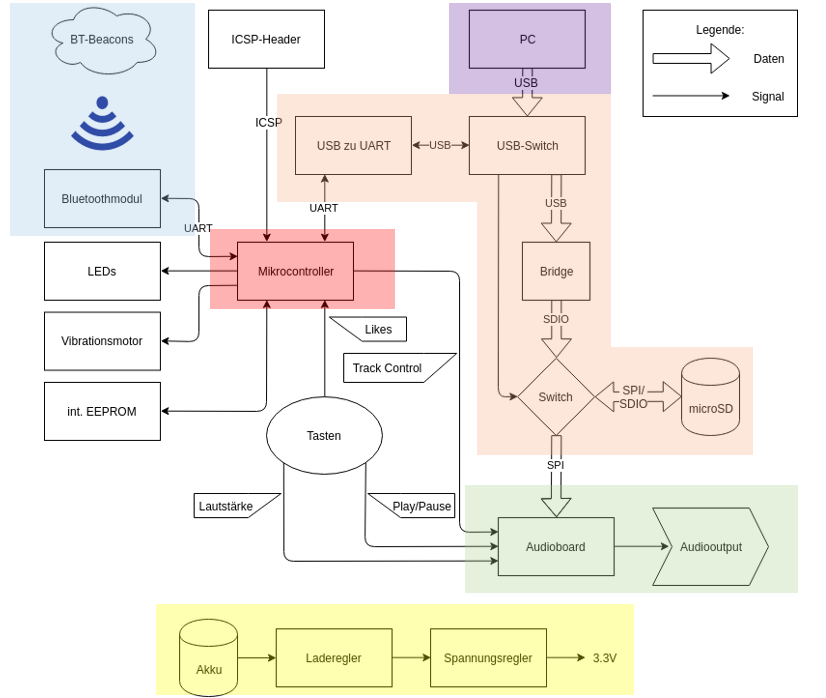
\includegraphics[width=14cm]{Bilder/Gesamtsystem.png}
	\caption{Blockschaltbild Gesamtsystem}
	\label{Blockschaltbild_Gesamtsystem}
\end{figure}

\begin{table}[h]
	\centering
	\begin{tabular}{|c|c|c|c|c|c|} 
		\cellcolor{myviolett}Software & \cellcolor{myyellow}Energieversorgung & \cellcolor{myorange}USB & \cellcolor{mygreen}Audioausgabe & \cellcolor{myblue}Bluetooth & \cellcolor{myred}Firmware \\ 
	\end{tabular} 
	\caption{Legende Gesamtsystem}
	\label{legend_gesamtsystem}
\end{table}

\chapter{Software}
\label{Software}
% ================ Einstellungen =======================
\thispagestyle{fancy} \rhead{\slshape Software}
% ======================================================
Im Kapitel Software wird erläutert, wie die Audiodateien auf das Dojo gelangen und die Korrespondenztabelle angepasst werden kann. Es wird erklärt, wie die Likes ausgewertet und verarbeitet werden können.

%\section{Konzept}
%In diesem Unterkapitel wird das erarbeitete Konzept für die Datenübertragung von einem Computer auf das Dojo dargelegt.

\section{Datenverwaltung}
Alle Ausstellungsobjekte sind in einer Textdatei aufgelistet, in der vermerkt wird, welche Audio- und Textdatei zu welchem Beacon gehört.
Die Form dieser Inventardatei ist in Abbildung \ref{inventory_syntax} zu sehen.

Zudem wird in einer weiteren Textdatei ein Preset definiert, mit der die $\mu$SD-Karte beschrieben werden kann.
Die Form dieser Presetdatei ist in Abbildung \ref{preset_syntax} zu sehen.

\begin{figure}[h]
	\begin{verbatim}
exhibition romans{
    233(
        de  roemischerhelm.mp3  roemischerhelm.tex
        en  romanhelmet.mp3     romanhelmet.tex
    )
    10(
        de  becher_rom.mp3      becher_rom.tex
        en  cup_rome.mp3        cup_rome.tex
    )
}

exhibition middle_ages{
    15(
        de  mittelalterlicher_schaedel.mp3  mittelalterlicher_schaedel.tex
        en  skull_medieval.mp3              skull_medieval.tex
    )
    11(
        de  morgenstern.mp3         morgenstern.tex
        en  primitive_weapon.mp3    primitive_weapon.tex
    )
}
	\end{verbatim}
	\caption{Inventardatei für eine Testausstellung}
	\label{inventory_syntax}
\end{figure}

\begin{figure}[h]
	\begin{verbatim}
languages: de, en
exhibitions: romans, middle_ages
	\end{verbatim}
	\caption{Presetdatei für eine Testausstellung}
	\label{preset_syntax}
\end{figure}

Der CLI-Befehl \texttt{makepackage} nimmt die Inventardatei und Presetdatei und generiert einen Ordner, in dem sich alle Audiodateien befinden, die in der Inventardatei aufgelisteten sind.
Die Dateien des generierten Audiopakets haben als Namen nur noch eine Zahl, die bestimmt an welcher Stelle sie auf der $\mu$SD-Karte abgespeichert wird.

Der CLI-Befehl \texttt{loadsd} nimmt das vorher generierte Audiopaket und schreibt es auf die $\mu$SD-Karte des Audioguides.
Dazu schickt es dem Mikrocontroller den Befehl, dass er den Multiplexer umschaltet.
Das Betriebssystem des PC sollte dann die $\mu$SD-Karte mounten und dem Python Skript verfügbar machen, worauf dieses die Daten kopiert.
Es wird dabei angenommen, dass nur ein Audioguide am PC angeschlossen ist und dass alle $\mu$SD-Karten "dojo-sd" heissen.

Der CLI-Befehl \texttt{maketicket} nimmt die Inventardatei und die Presetdatei als Argumente und fragt den Nutzer, welche Ausstellungen dem Besucher in welcher Sprache zur Verfügung stehen sollen. 
Mit diesen Inputs wird ein Ticket generiert, das über die serielle Schnittstelle auf das EEPROM des Mikrocontrollers geladen wird.

Auf dem EEPROM des Dojos sind jedem Beacon zwei Bytes zugeordnet, die die Beacon-ID, Like- und Zutrittsinformation beinhalten.
Die Likes sind zu Beginn des Besuchs alle auf null und können vom Besucher gesetzt werden.
Die Zutrittsbits der bezahlten Ausstellungen werden zu Beginn des Besuchs gesetzt und können vom Besucher nicht verändert werden.

% In diesem Kapitel wird beschrieben wie die Konfigurationsdateien ausgelesen werden. Zudem wird die Korrespondenztabelle erläutert. 

\section{Auslesen, Schreiben}
Das EEPROM des Mikrocontrollers wird über eine serielle Schnittstelle beschrieben, wobei alle Befehle das gleiche Muster haben:
\begin{verbatim} [1 char] op-code | [3 char] arg1 | [3 char] arg2 ; \end{verbatim}
Um ein Byte mit Wert 42 in die Adresse 2 zu schreiben, muss der String \texttt{p002042} auf die serielle Schnittstelle geschrieben werden.
Um das Byte an der Adresse 2 auszulesen, muss der String \texttt{r002   ;} auf die serielle Schnittstelle geschrieben werden.
Wichtig ist, dass alle Befehle mit einem Semikolon terminiert werden.

Das Python Modul beinhaltet neben Schreib- und Lesefunktionen auch noch Funktionen, die ein ganzes Ticket auf das EEPROM schreiben bzw. wieder einlesen können.
Hier ist es wichtig, dass das vordefinierte Muster des EEPROMs in Abbildung \ref{eeprom_memory_pattern} eingehalten wird.


\begin{figure}
	\begin{tabular}{l|l}
		Anzahl gespeicherter Beacons & Sprachcode                      \\ \hline
		ID Beacon1                   & Like Beacon1, Zutritt Beacon1   \\ \hline
		ID Beacon2                   & Like Beacon2, Zutritt Beacon2   \\ \hline
		\(\vdots\)                   & \(\vdots\) 
	\end{tabular}
	\caption{EEPROM Adressierungsmuster}
	\label{eeprom_memory_pattern}
\end{figure}
% Hier wird beschrieben wie die Verbindung und die Datenübertragung auf den internen EEPROM realisiert wird.

\section{Validierung}
Für die Validierung der Datenverwaltung wurden Python Unittests eingesetzt, die mit einer Testdatenbank alle Funktionen testen.
Neben den einzelnen Funktionen wurde auch ein kompletter Durchlauf mit der Testdatenbank gemacht.

Die EEPROM-Operationen werden mit einem Arduino Uno-Board getestet, wobei das EEPROM vom PC aus beschrieben und wieder eingelesen wird.
Die Unittests stellen sicher, dass das EEPROM die gewünschten Daten beinhaltet und dass diese mit der spezifizierten Geschwindigkeit übertragen werden.

Es werden zudem Benchmarks durchgeführt, welche sicherstellen, dass nicht unnötig gewartet wird.
Ein Test, der misst wie lange das Beschreiben von verschieden langen Tickets dauert, zeigt, dass das Beschreiben eines vollen Tickets mit 250 Beacons $6.17s$ dauert.
% Hier werden die Python Unittests, welche verwendet wurden, dargelegt.


\chapter{Energieversorgung}
\label{Energieversorgung}
% ================ Einstellungen =======================
\thispagestyle{fancy} \rhead{\slshape Energieversorgung}
% ======================================================

Wie in allen Bereichen des vorliegenden Projekts geht es auch im Bereich der Energieversorgung darum, aus dem verfügbaren Raum, kosteneffizient eine möglichst gute Performance zu erhalten. Um dies zu gewährleisten, muss der Energiebedarf der Elektronik auf ein Minimum reduziert werden. Mit der Auswahl von energieeffizienten Komponenten und einem effizienten Ablauf im Programmcode, kann dem entgegengewirkt werden. Der Energiebedarf von Komponenten, die gerade nicht in Verwendung sind, kann so erheblich reduziert werden. Wird zum Beispiel der Mikrocontroller nicht aktiv verwendet, versetzt er sich in einen energiesparenden Bereitschaftsmodus, der einen wesentlich geringeren Verbrauch hat.

\section{Technische Grundlagen}
 
Die maximale Grösse des Akkus war durch das designte Gehäuse bereits vorgegeben. Somit konnte eine einfache Auswahl getroffen werden. Um den Energiebedarf des Dojos abzuschätzen, wurde zu Beginn der Projektarbeit eine Energiebedarfsberechnung anhand von Datenblattangaben der verwendeten Komponenten gemacht. Die Berechnungen haben gezeigt, dass das Wunschziel, die Akkulaufzeit des Dojos auf einen ganzen Museumstag auszulegen, ins Auge gefasst werden kann. Dies führt im Museum zu einer hohen Verfügbarkeit solcher Geräte.  Das Museum benötigt so wesentlich weniger Geräte und muss nicht ständig die Geräte auswechseln und aufladen. Ausserdem verringert sich der Arbeitsaufwand, da die Dojos nicht in jeder freien Minute ins Ladegerät gesteckt werden müssen, sondern ein Ladezyklus über Nacht ausreicht.\\

Die ursprüngliche Energiebedarfsberechnung der wichtigsten Komponenten hat bei einer durchschnittlichen Nutzung von zehn Stunden einen Speicherbedarf von 400 mAh ergeben. Es wurde angenommen, dass das Dojo während einem Drittel der Zeit aktiv genutzt und in der übrigen Zeit in Standby-Modus versetzt wird. 



%In diesem unter Kapitel werden die technischen Grundlagen für das Verständnis der Energieversorgung dargelegt.
\section{Konzept}
Hier wird das verwendete Konzept der Energieversorgung respektive der Ladeschaltung erklärt und begründet. 
\section{Hardware}
Hier steht welche Bauteile in welcher Anordnung verwendet wurden.
\section{Validierung}
Hier wird erklärt, wie die Validierung der Ladeschaltung gelöst wurde. Die Resultate der Validierung (der Energieversorgung) und die eventuellen Abweichungen zu den Wünschen werden in diesem Kapitel beschrieben.

\chapter{USB}
% ================ Einstellungen =======================
\thispagestyle{fancy} \rhead{\slshape USB} 
% ======================================================
\section{Technische Grundlagen}
\section{Konzept}
\section{USB zu UART}
\section{USB zu SDIO}
\section{Validierung}
\chapter{Audioausgabe}
\label{Audioausgabe}
% ================ Einstellungen =======================
\thispagestyle{fancy} \rhead{\slshape Audioausgabe} 
% ======================================================
In diesem Kapitel werden die technischen Grundlagen welche sich auf das verwendete Audio-Modul beziehen, das Konzept sowie die Funktion der Audioausgabe beschrieben. Zudem wird die Validierung erläutert.
\section{Technische Grundlagen}\label{TechWTV}
Das Konzept von Dojo sieht als Abspielgerät der Audiodateien einen Bone Conductor vor. Der Bone Conductor sowie das für den Prototyp verwendete Audio Modul WTV020 werden in diesem Kapitel beschrieben. Diese Informationen werden in den nachfolgenden Kapiteln benötigt. 
\paragraph{WTV020}
Das WTV020 Modul ist ein Soundmodul welches es ermöglicht, Audiodateien auf einem Aktor abzuspielen. Auf einer maximal 1GB grossen $\mu$SD-Karte können bis zu 512 Audiodateien abgespeichert werden. Die Audiodateien auf der $\mu$SD-Karte müssen jedoch dem .wav oder .ad4 Format entsprechen. Die Dateien müssen gemäss Vorgabe: 0000; 0001; 0002; … nummeriert werden.\\
Der WTV020 Chip kann in zwei verschiedenen Modes betrieben werden, dem MP3 Mode und dem Two Line Serial Mode. Im MP3 Mode können direkt 6 Pins angesteuert werden. Durch die sechs Pins können folgende Funktionen umgesetzt werden: Reset, $\pm$Volume , next, previous und play, pause. 
Für das Dojo wird jedoch der two line serial mode genützt. Dieser kann das Modul mit nur 3 Pins betreiben. Der Mikrocontroller muss an den Clock-, den Data- und den Busy-Pin angeschlossen werden. Im two line serial mode können die Audiodateien welche sich auf der $\mu$SD-Karte befinden abgespielt werden. Er ermöglicht zudem, ähnlich wie im MP3 Mode ein Lied zu pausieren und neu zu starten, sowie eine Lautstärkenregulation. \cite{WTV020}

\paragraph{Bone Conductor}
Die Audioausgabe erfolgt wie beschrieben über einen Bone Conductor. Der Bone Conductor besteht aus einem kleinen Metallstab, welcher mit einer Kupfer Spule umwickelt ist. Sobald ein pulsförmiger Strom durch die Spule fliest, dehnt sich ein Magnetfeld aus welches die benötigten Vibrationen auf ein flaches Metallstück auslöst. 
\begin{figure}[h]
	\centering
	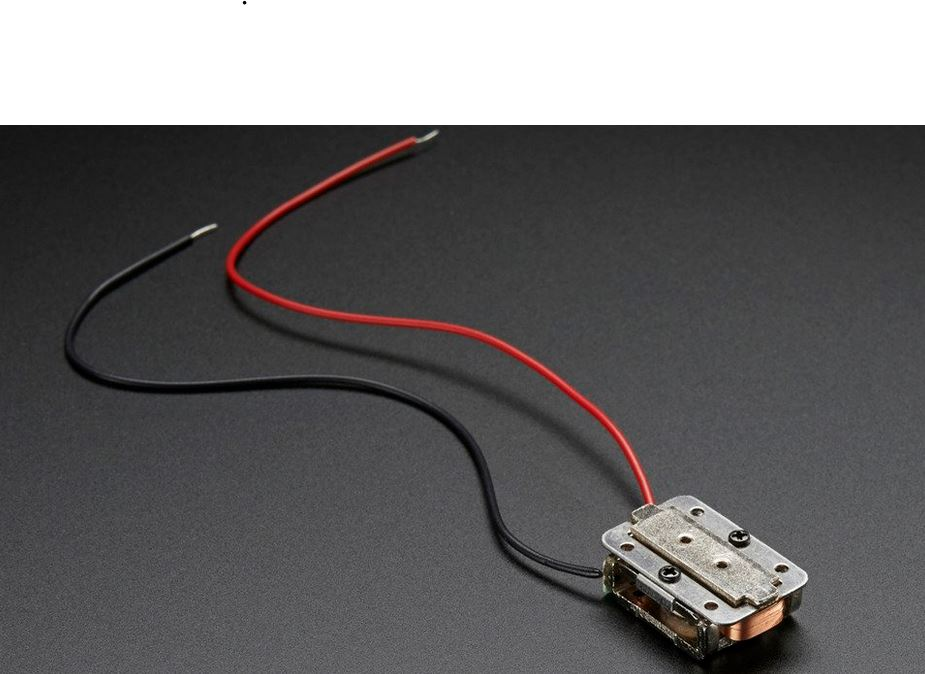
\includegraphics[width=6cm]{Bilder/Bone-Conductor.jpg}
	\caption[Bone Conductor]{Bone Conductor \cite{BoneConductor}}
	\label{Bone-Conductor}
\end{figure}

In der Abbildung \ref{Bone-Conductor} ist der für den Dojo benötigten Bone Conductor abgebildet. Der Bone Conductor ermöglicht es durch die Vibrationen, dass eine Audio Datei über den Schädelknochen abgespielt wird und so nur für eine Person hörbar ist, diese jedoch immer noch die Umgebungsgeräusche wahrnimmt. \cite{BoneConductor}



\section{Konzept}\label{AudioKonzept}
Das Konzept der Audioausgabe ist wie folgt aufgebaut:
\begin{figure}[h]
	\centering
	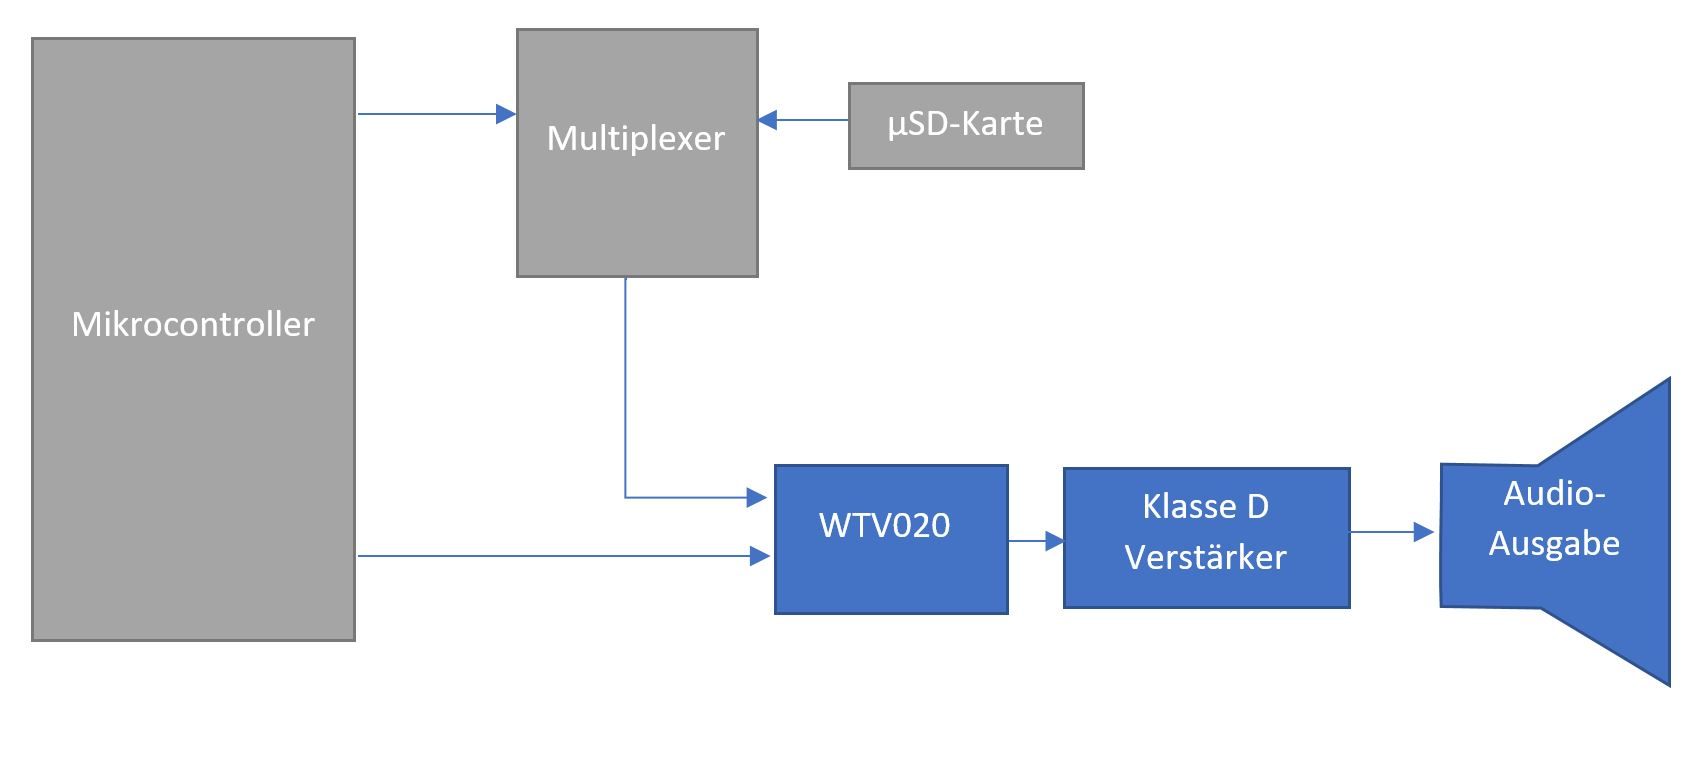
\includegraphics[width=11cm]{Bilder/Audio-Konzept.jpg}
	\caption{Audio Konzept}
	\label{Audio-Konzept}
\end{figure}\\
Die auf einer $\mu$SD-Karte abgespeicherten Audiodateien werden über einen Multiplexer, welcher vom Mikrocontroller gesteuert wird, an einen WTV020 Chip übertragen. Dieser wird in einem Serial Mode \ref{TechWTV} betrieben und kann ebenfalls vom Mikrocontroller angesteuert werden. Der Audiochip entschlüsselt die Daten und gibt diese an einen Klasse D Verstärker weiter. Dieser wird benötigt, um eine gut hörbare Lautstärke zu erreichen. Das Audiosignal wird schliesslich an einem Bone Conductor ausgegeben. 
Nachfolgend wird die Anordnung auf dem Print der einzelnen Komponenten dargelegt. 
\section{Hardware}
Wie im Konzept \ref{AudioKonzept}
 beschrieben, muss man, um Daten von der $\mu$SD-Karte auszulesen zuerst den Multiplexer ansteuern. Dies geschieht über den Mikrocontroller. Im ungesteuerten Zustand ist der MUX auf den WTV020-Chip geschaltet. Der WTV020SD-20S Chip kann nun auf die $\mu$SD-Karte zugreifen. Über vier Pins werden die Audiofiles ausgelesen und weitergegeben. Das Audiosignal wird auf den Klasse-D Verstärker gegeben. Dieser ist wie folgt aufgebaut.
\begin{figure}[h!]
	\centering
	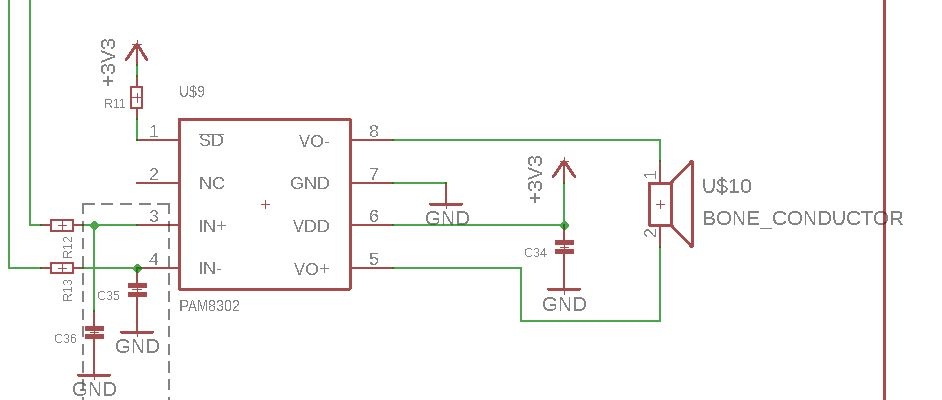
\includegraphics[width=10cm]{Bilder/Klasse-D.jpg}
	\caption{Klasse D Verstärker}
	\label{Klasse-D}
\end{figure}


Um ein Rauschen an der Speisung zu vermeiden, wird ein 1$\mu$ Farad grosser Kondensator benötigt. In diesem Projekt wurde zuerst eine konstante Verstärkung mit dem Faktor ca.10 verwendet, da die Lautstärken Regelung über den WTV020-Chip geregelt werden soll. Dieser Faktor entsteht aus dem Verhältnis des Internen Widerstandes und den zugeschalteten Widerständen. Um das Rauschen der Eingänge, sowie zu hohe Frequenzen zu filtern wurden zuerst wie die Abbildung \ref{Klasse-D} zeigt, Kapazitäten eingeplant. Auf dem Prototyp wurden aufgrund von Tests welche in der Validierung aufgeführt werden, die Vorwiderstände durch Kapazitäten ersetzt und die geplanten Kapazitäten weggelassen.\\ Wie erwähnt wird die Lautstärkenregelung über den WTV020-Chip geregelt. Dies ist jedoch im serial mode fehleranfällig. Übergangsweise wurde um die Lautstärke zu dämmen ein 50 Ohm grosser Widerstand vor den Bone Conductor geschaltet. Die Audioausgabe kann also wie beschrieben mit dem Bone Conductor umgesetzt werden.

\section{Firmware}
Wie im Kapitel Hardware beschrieben muss der MUX angesteuert werden um dem WTV-Chip den Zugriff auf die $\mu$SD-Karte zu gewähren. Im Kapitel \ref{USB} in der Tabelle \ref{truth_table_sd} ist beschrieben wie der MUX angesteuert werden muss, damit die benötigten Pins durchgeschaltet sind.
Für die Audioausgabe müssen alle Öffner geschlossen werden. Dies wird über die Pins 25 – 27 (Port C) realisiert. Sobald Musik abgespielt werden muss, werden die benötigten Ausgänge gesetzt. Das  WTV020 Modul vergleicht die Daten und Clock Pins wie folgt :
\begin{figure}[h]
	\centering
	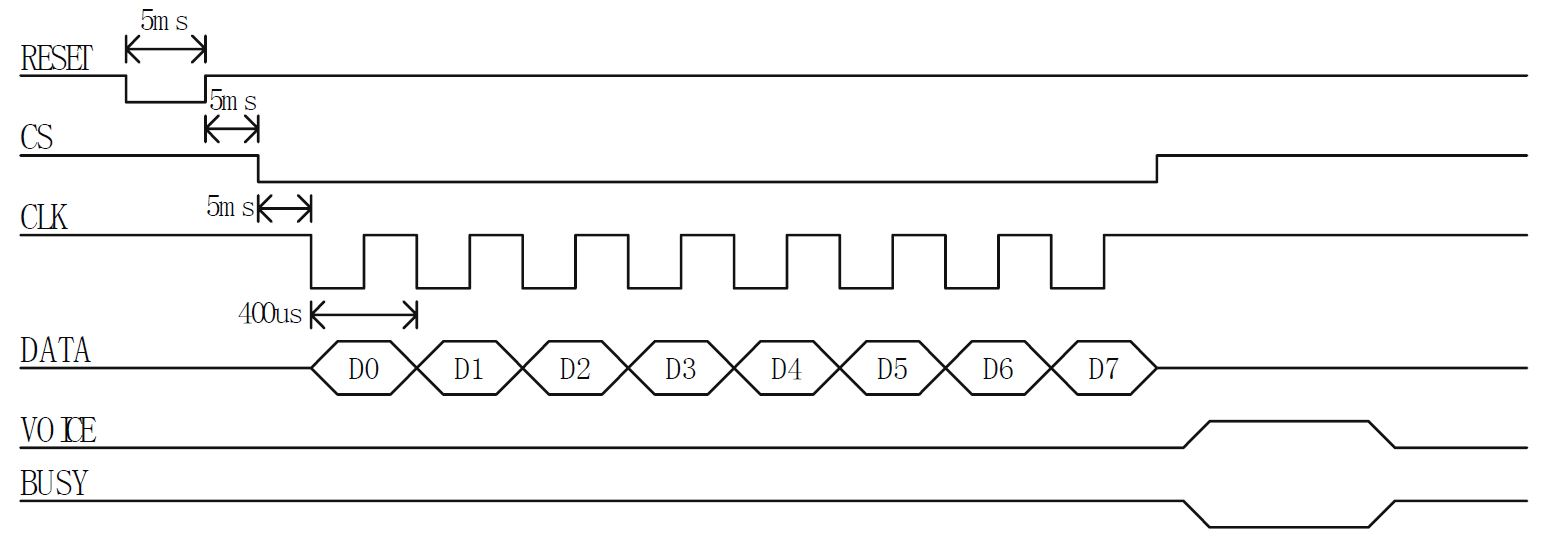
\includegraphics[width=15cm]{Bilder/WTV-Serial-Mode.JPG}
	\caption{WTV Serial Mode}
	\label{WTV-Serial}
\end{figure}\\
In der Abbildung \ref{WTV-Serial} ist ein three line serial mode dargestellt. Für den benötigten two line serial mode wird der CS Pin nicht benötigt.
\newpage
Sobald am Pin 7 über einen Taster Play ein low Signal erkannt wird, wird folgende Funktion aufgerufen:

\begin{figure}[h]
	\begin{verbatim}
void sendWTVcommand(unsigned int command){
	digitalWrite(WTV_CLK, LOW);
	_delay_us(1900);
	for (byte i = 0; i < 16; i++)
	{
		_delay_us(100);
		digitalWrite(WTV_CLK, LOW);
		digitalWrite(WTV_DOUT, LOW);
		if ((command & 0x8000) != 0)
		{
			digitalWrite(WTV_DOUT, HIGH);
		}
		_delay_us(100);
		digitalWrite(WTV_CLK, HIGH);
		command = command<<1;
	}
}
	\end{verbatim}
	\caption[Audio Datei abspielen]{Audio Datei abspielen \cite{WTVCODE}}
	\label{WTV-Play}
\end{figure}


Die benötigten Befehle welche sendWTVcommand mitgegeben werden müssen sind aufgrund des WTV020-Chips vorgefertigt.
Nachfolgend werden die verwendeten Befehle und deren Funktion aufgeführt.\\

	
\begin{table}[h]
	\centering
	\begin{tabular}{|c|c|} 
		Funktion & Befehl\\ 
		\hline 
		Play\_Pause & 0xFFFE \\ 
		\hline 
		STOP & 0xFFFF \\ 
		\hline 
		VOL & 0xFFF0-0xFFF7 \\ 
	\end{tabular} 
	\caption{WTV020 Funktionen}
	\label{WTVFunktionen}
\end{table} 

Bei der Funktion Play\_Pause ist zu erwähnen, dass um die Ausgabe zu starten am Anfang die gewünschte File Nummer gesendet werden muss (0-512). Ohne File Nummer wird die aktuelle Audioausgabe pausiert und kann wieder gestartet werden.

\section{Validierung}
Um die Audioausgabe zu testen, wurden verschiedene Versuche durchgeführt. Zuerst wurde der Bone Conductor über eine kleine Verstärkerschaltung direkt an einem Laptop angeschlossen, um die benötigte Leistung und die Lautstärke abschätzen zu können. Bei diesen Messungen ergab sich, bei einer sehr gut hörbaren Lautstärke, eine maximale Scheinleistung von 0.28 VA.\\
Um das WTV020 Modul mit geringem Aufwand zu testen wurde dieses zuerst im MP3 Mode betrieben.
So konnten schon am Anfang nicht kompatible $\mu$SD-Karten aussortiert werden. \\
Alle Funktionen des WTV020-Chips wurden separat und im two line serial mode überprüft. Alle verlangten Funktionen des Chips laufen Wunschgemäss. Zudem wurde ein Versuchsaufbau mit dem D-Klasse Verstärker durchgeführt, mit welchem die aktuell maximal benötigte Leistung von 1W gemessen wurde. \\
Trotz der funktionierenden Tests ist aktuell am Prototyp die Lautstärkenregelung nicht möglich. Das Audiomodul übernimmt die eingestellte Lautstärke, setzt diese jedoch, sobald das Gerät an einen Verstärker angeschlossen ist, vorherigen Wert zurück. Zudem ist zu erwähnen, dass für eine Massenproduktion ein WTV020 Modul nicht geeignet wäre, aufgrund der erwähnten Eigenheiten. Das Modul nimmt trotz gleicher Formatierung und gleichem Hersteller nicht jede $\mu$SD-Karten an. Zudem treten beim serial mode immer wieder kleiner Ungereimtheiten auf, wie z.B. die Lautstärkenregelung. 

\chapter{Bluetooth}
% ================ Einstellungen =======================
\thispagestyle{fancy} \rhead{\slshape Einleitung} \setcounter{page}{1} \cfoot{\thepage} \renewcommand{\footrulewidth}{0.4pt} 
% ======================================================
\section{Technische Grundlagen}
\section{Konzept}
\section{Hardware}
\section{Firmware}
\section{Validierung}

\chapter{Firmware}
\label{Firmware}
% ================ Einstellungen =======================
\thispagestyle{fancy} \rhead{\slshape Firmware}
% ======================================================
Die Firmware wurde auf einen ATMega 328p Mikrochip geflashed (siehe Abbildung \ref{fig:ATMega328p}). Für die Kommunikation (UART) mit dem Bluetoothmodul ist eine zusätzliche Softwareserial (Pins PD2 \& PD3) zur üblichen seriellen Schnittstelle (Pins PD0 \& PD1) implementiert, da der ATMega 328p nur ein UART Interface (TXD \& RXD) auf den Pins PD0 \& PD1 hat. Der ATMega 328p wird mittels einem ISP (AVR-Dragon) über den sechs poligen ICSP-Header (Anhang: Schema Sheet: 3/3) JP1 geflashed.\\
Folgende Einstellungen wurden im Device Programming unter Fuses im AtmelStudio dafür vorgenommen:
\begin{itemize}
\item EXTENDED.BODLEVEL: Brown-out detection disabled
\item HIGH.SPIEN: enabled
\item HIGH.BOOTZ: Boot Flash size=2048 words start address=\$3800
\item LOW.SUT\_CKSEL: Ext. Crystal Osc. 8.0- MHz; Start-up time PWRDWN/RESET: 1K CK /14 CK + 65ms
\item EXTENDED: 0xFF
\item HIGH: 0xD9
\item LOW: 0xCF
\end{itemize}
\begin{figure}[h]
\centering
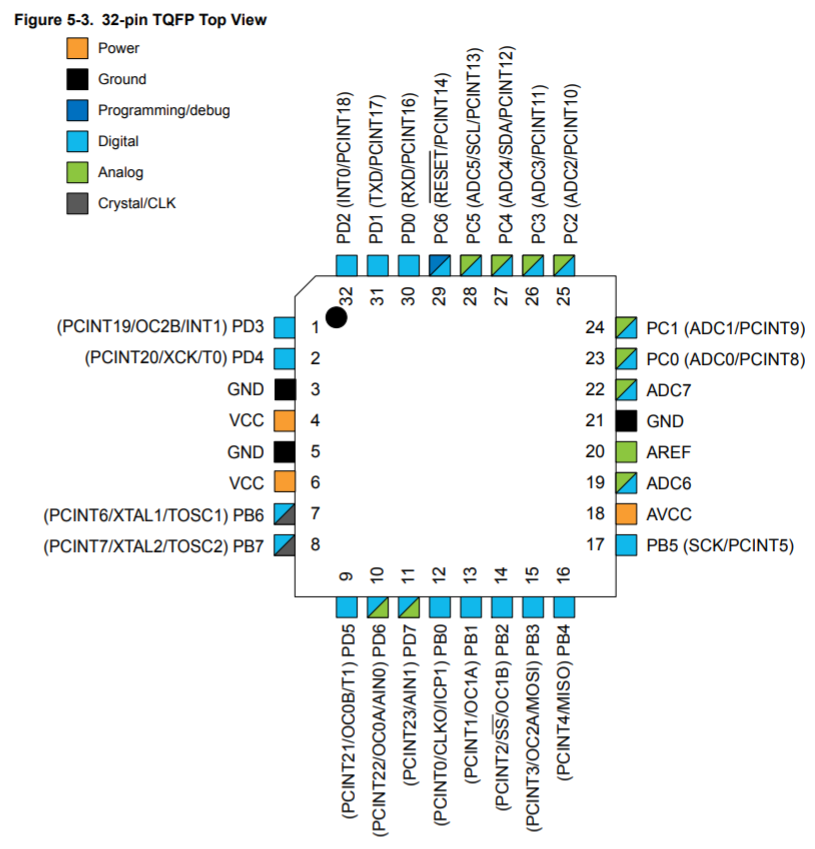
\includegraphics[width=0.59\textwidth]{Bilder/atmega328p.png} 
\caption[ATMega 328p]{ATMega 328p \cite{atmega328p}}
\label{fig:ATMega328p}
\end{figure}
\newpage
Die Firmware ist so designed, dass alle $\sharp defines$, die extern foreward declarated Funktionen und alle weiteren inkludierten Headerfiles in der Dojo.h Datei implementiert sind. Diese wird dann von der Dojo\_Functions.cpp und der Sketch.cpp Datei eingebunden. In der Abbildung \ref{fig:uml_diagramm} ist der allgemeine Aufbau der Firmware in einem UML-Diagramm visualisiert.\\
\begin{figure}[H]
\centering
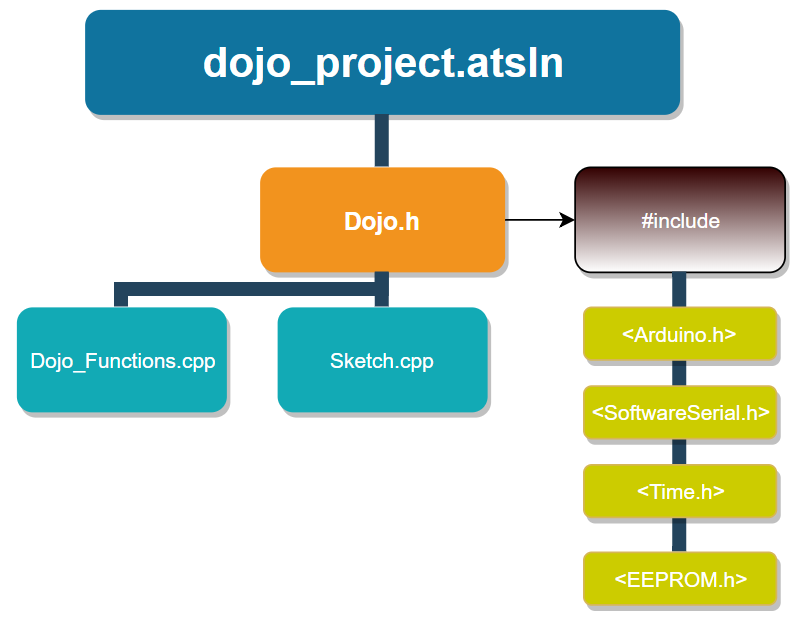
\includegraphics[width=0.8\textwidth]{Bilder/uml_diagramm.PNG} 
\caption{UML-Diagramm Firmware}
\label{fig:uml_diagramm}
\end{figure}
In der Tabelle \ref{tab:auslastung} ist die Auslastung des ATMegas mit der Endversion der geflashten Firmware dargestellt. Diese ist relativ niedrig und bietet für einen weiteren Aufbau genügend freie Memory.\\
\begin{table}[H]
\centering
\begin{tabular}{|l|r|r|}
\hline 
Program Memory Usage: & 5064 bytes & 15.5 \% Full \\ 
Data Memory Usage: & 429 bytes & 20.9 \% Full \\ 
\hline 
\end{tabular} 
\caption{Auslastung des ATMega 328p}
\label{tab:auslastung}
\end{table}
\newpage
\section{Statemachine}
Auf dem Mikrocontroller läuft eine Mealy-Statemachine mit sechs Zuständen (siehe Abbildung \ref{fig:mealy_statemachine}):\\
\begin{itemize}[leftmargin=3.2cm]
\item[INIT:] Hier wird das setup() der Firmware ausgeführt. Dabei werden alle nötigen Pinkonfigurationen initialisiert und und das WTV-Modul konfiguriert.
\item[SCAN:] Es wird vom Dojo nach IBeacons in naher Umgebung gesucht. Falls einer gefunden wurde, dann wird direkt das dazugehörige Audiofile bereitgestellt. Wird der Playbutton gedrückt, ändert sich der State zu PLAY. Ansonsten wird weiter gescanned.
\item[PLAY:] Hier werden die bereitgestellten Audiofiles abgespielt. Wird der Playbutton nochmals gedrückt, wird das Abspielen abgebrochen und der State wechselt wieder zu SCAN.
\end{itemize}
Wird das Dojo an den Computer angeschlossen, ist der Zustand des Dojos abhängig von der gewünschten Tätigkeit. Dafür wird vom Computer aus ein Befehl über das USB-Kabel gesendet, woraufhin sich der State ändert:
\begin{itemize}[leftmargin=3.2cm]
\item[GET\_LIKES:] Die vom Besucher getätigten Likes werden vom EEPROM auf den Computer transferiert.
\item[LOAD\_SD:] Sobald das Dojo in diesem State ist, schaltet der Multiplexer um und die $\mu$SD-Karte kann wie ein normaler Datenträger beschrieben werden.
\item[LOAD\_CONFIG:] Ein Ticket wird auf das interne EEPROM geladen.
\end{itemize}
\begin{figure}[h]
\centering
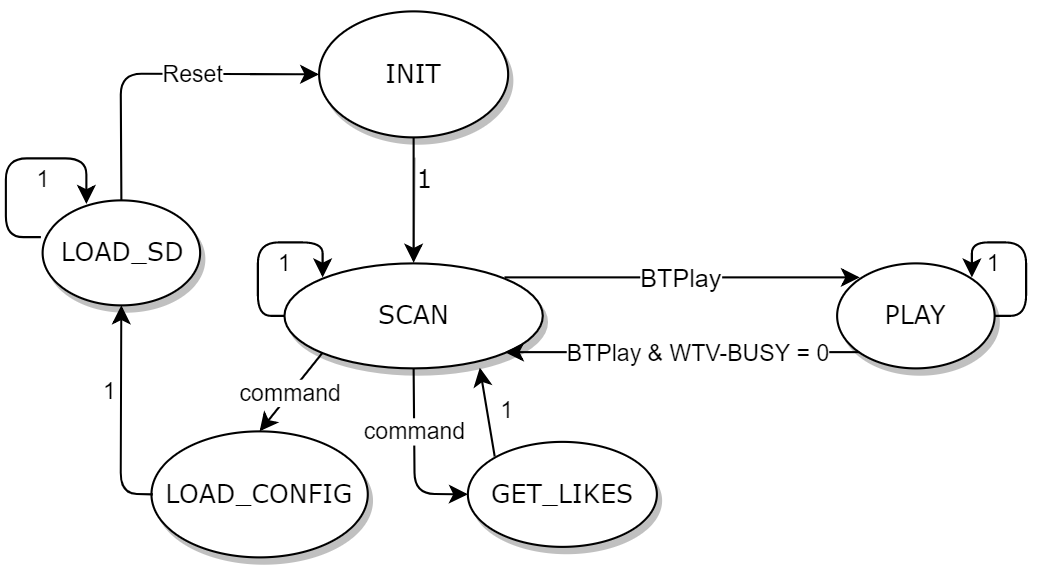
\includegraphics[width=0.9\textwidth]{Bilder/statemachine.PNG} 
\caption{Mealy-Statemachine}
\label{fig:mealy_statemachine}
\end{figure}
\newpage
 \section{Datenverwaltung}
%In diesem Kapitel wird die Datenverwaltung auf dem internen EEPROM erklärt.
Das Ticket auf dem EEPROM beinhaltet für jedes Ausstellungsobjekt zwei Bytes, das erste beinhaltet die Beacon-ID und das zweite das Zutritts- und Like-Bit.
Die ersten zwei Bytes sind reserviert und beinhalten die Anzahl gespeicherter Beacons und ein Sprachcode: 0 für die erste Sprace, 1 für die zweite.
Da auf der $\mu$SD-Karte die Dateien der zwei Sparchen abewechslungsweise und in gleicher Reihenfolge wie im EEPROM aufgelistet sind, muss nur der Index der Beaon-ID übergeben werden damit die korrekte Audiodatei abgespielt werden kann: \\
\texttt{(BeaconIndex - 2) * 2 + Sprachcode}.
\section{Validierung}
%Hier wird die Validierung der kompletten Firmware sowie dessen Ergebnisse dargelegt. 
Die Validierung der Datenverwaltung wurde mit Unittests vom PC aus gemacht. Dabei wurde ein mit Zufallszahlengenerator generiertes Ticket über die serielle Schnittstelle auf das EEPROM geschrieben und dann wieder eingelesen. Diese Validierung wurde direkt auf dem Arduino UNO Board gemacht und hat funktioniert.
\\[0.5cm]
Auf dem MCU sind am Ende noch Probleme beim Auslesen des Receivebuffer von der seriellen Schnittstelle über das USB-Kabel zum Computer aufgetaucht. Dabei konnten über mySerial.available() die vom Computer gesendeten Befehle nicht ausgelesen werden. Mit dem Oszilloskop sind die gesendeten Befehle auf dem PD0 zwar messbar, allerdings können von der Seite des MCUs aus diese \glqq Daten\grqq\; nicht detektiert werden. Deshalb funktioniert die Kommunikation vom Computer zum MCU auf dem Prototyp nicht wie geplant. Umgekehrt vom MCU zum Computer können aber Daten gesendet werden. Um die States zu ändern, wurden nun für die gesamte Funktion Taster zur Stateänderung verwendet, damit die Statemachine und der Ablauf der Firmware funktioniert.
\\[0.5cm]
Dabei sind die Tasterfunktionen:
\begin{itemize}[leftmargin=1.2cm]
\item[SW1:] Ändert den State zu LOAD\_SD
\item[SW2:] Ändert den State zu PLAY
\item[SW3:] Ändert den State zu LOAD\_CONFIG
\end{itemize}
Ein weiterer Aspekt, welcher dazu führt, dass für einen nächsten Prototyp des Dojos möglicherweise ein anderer Mikrochip benutzt wird ist, dass der ATMega 328p nur zwei external Interrupts hat (Abbilung \ref{fig:ATMega328p} Pins PD2-INT0 \& PD3-INT1). Diese sind momentan aber mit der Softwareserial belegt, weshalb mit den Taster nicht auf diese zugegriffen werden kann. Genauso gab es Konflikte mit der Softwareserial Library, die Tasterinterrupts über Pin Change Interrupts anzusteuern. Darum werden jetzt für die gesamte Funktion des Prototyps die Taster nach jedem scan() abgefragt und die Statusled zum togglen gebracht, wenn der Taster detektiert wurde.
\\[0.5cm]
Die $\mu$SD-Karte kann als normaler Datenträger mit den Audiofiles beschrieben werden. Zu beachten ist einfach, dass dies nur über einen Computer mit Linux als Betriebssystem funktioniert.

\chapter{Verzeichnisse}
% ================ Einstellungen =======================
\thispagestyle{fancy} \rhead{\slshape Verzeichnisse}
% ======================================================
\makeatletter
\renewcommand\chapter{\thispagestyle{\chapterpagestyle}%
                    \global\@topnum\z@
                    \@afterindentfalse
                    \secdef\@chapter\@schapter}
\makeatother
\listoffigures
\thispagestyle{fancy}
\newpage
\bibliography{Literaturverzeichnis/lit_fachbericht}
\thispagestyle{fancy}

\chapter{Anhang}
\label{Anhang}
% ================ Einstellungen =======================
\thispagestyle{fancy} \rhead{\slshape Anhang} 
% ============================================
\begin{figure}[h]
\centering
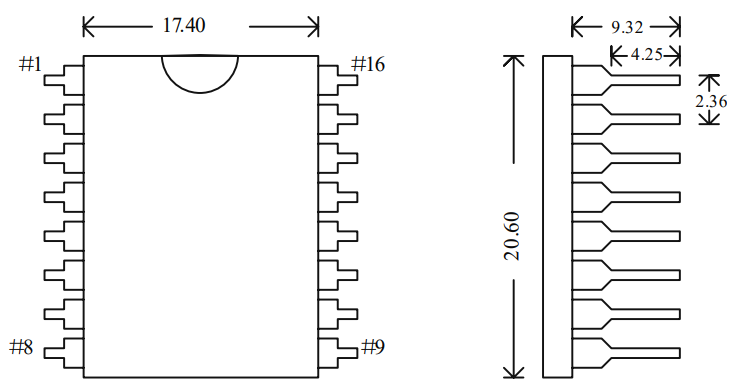
\includegraphics[scale=0.5]{Bilder/footprint_wtv020.png}
\label{fig:irgendesBild}
\caption[Abmessungen WTV020]{Abmessungen WTV020}
\end{figure}

\section{Benutzeranleitung}
\subsection{\texttt{maketicket inventory\_file preset\_file}}
Dieser CLI-Befehl schreibt ein "Ticket" auf das EEPROM.
Das inventory\_file beschreibt die ganze Datenbank, 
das preset\_file beschreibt, welche Audiodateien sich schon auf der SD-Karte befinden.
Gibt man den Befehl ein, promptet das Programm den Nutzer, 
welche Ausstellungen bezahlt sind und anschliessend welche Sprache gewünscht ist.
Sind diese Daten erfasst schreibt das Programm das Ticket über die serielle Schnittstelle auf das EEPROM.
\subsection{\texttt{makepackage inventory\_file preset\_file package\_path}}
Dieser CLI-Befehl kopiert die Audiodateien aller in der Presetdatei spezifizierter Ausstellungen in den Ordner package\_path. 
Die Dateien sind dann alle umbenannt, damit sie in der richtigen Reihenfolge auf die SD-Karte geschrieben werden.
\subsection{\texttt{loadsd package\_path}}
Dieser CLI-Befehl schreibt alle Audiodateien im Ordner package\_path auf die SD-Karte des Dojos. Alle schon auf der SD-Karte vorhandenen Dateien werden dabei gelöscht.

\newpage
Auf den folgenden Seiten befinden sich das Schema, das Layout und der Bestückungsplan der Printplatte.

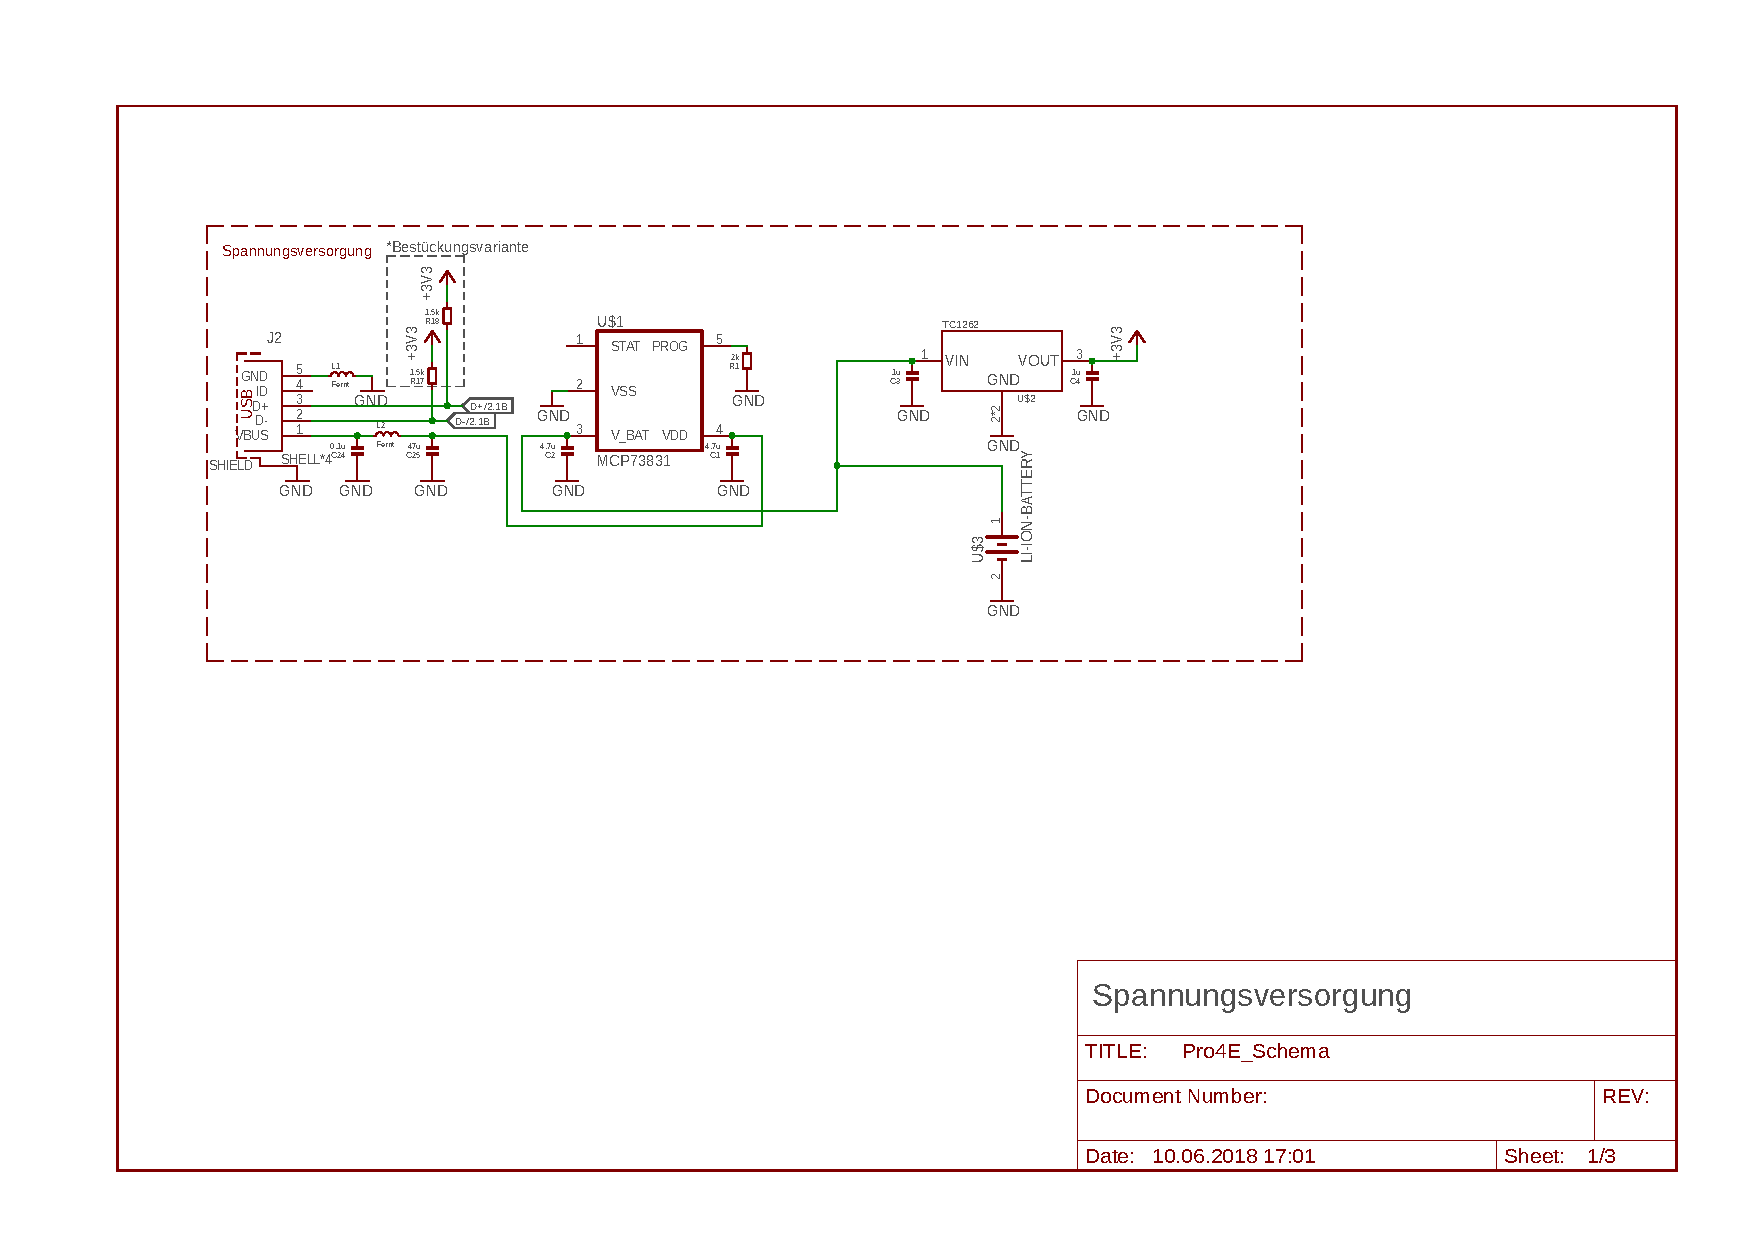
\includepdf[pages=1,fitpaper]{pdfs/Schema_Spannungsversorgung}
\label{pdf:SchemaSpannungsversorgung}

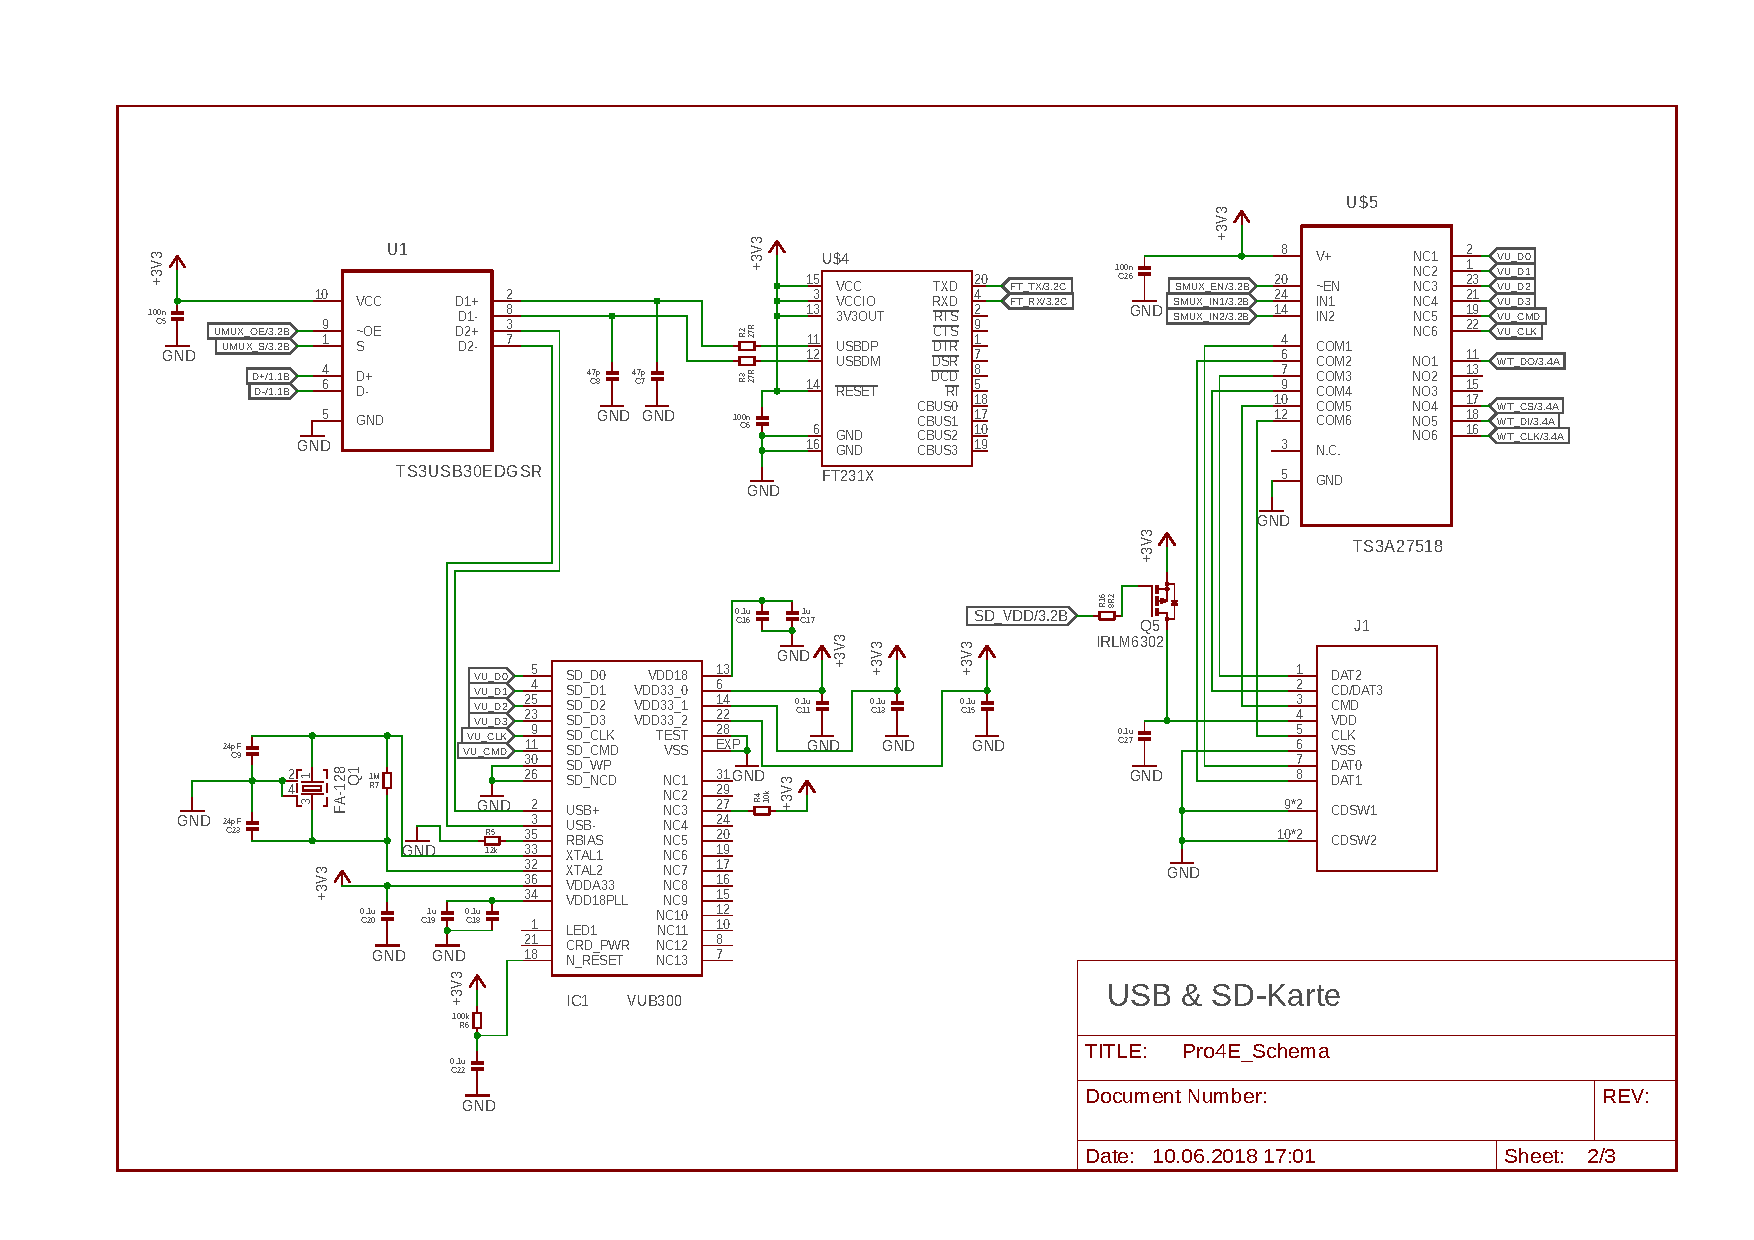
\includepdf[pages=1,fitpaper]{pdfs/Schema_USB}
\label{pdf:SchemaUSB}

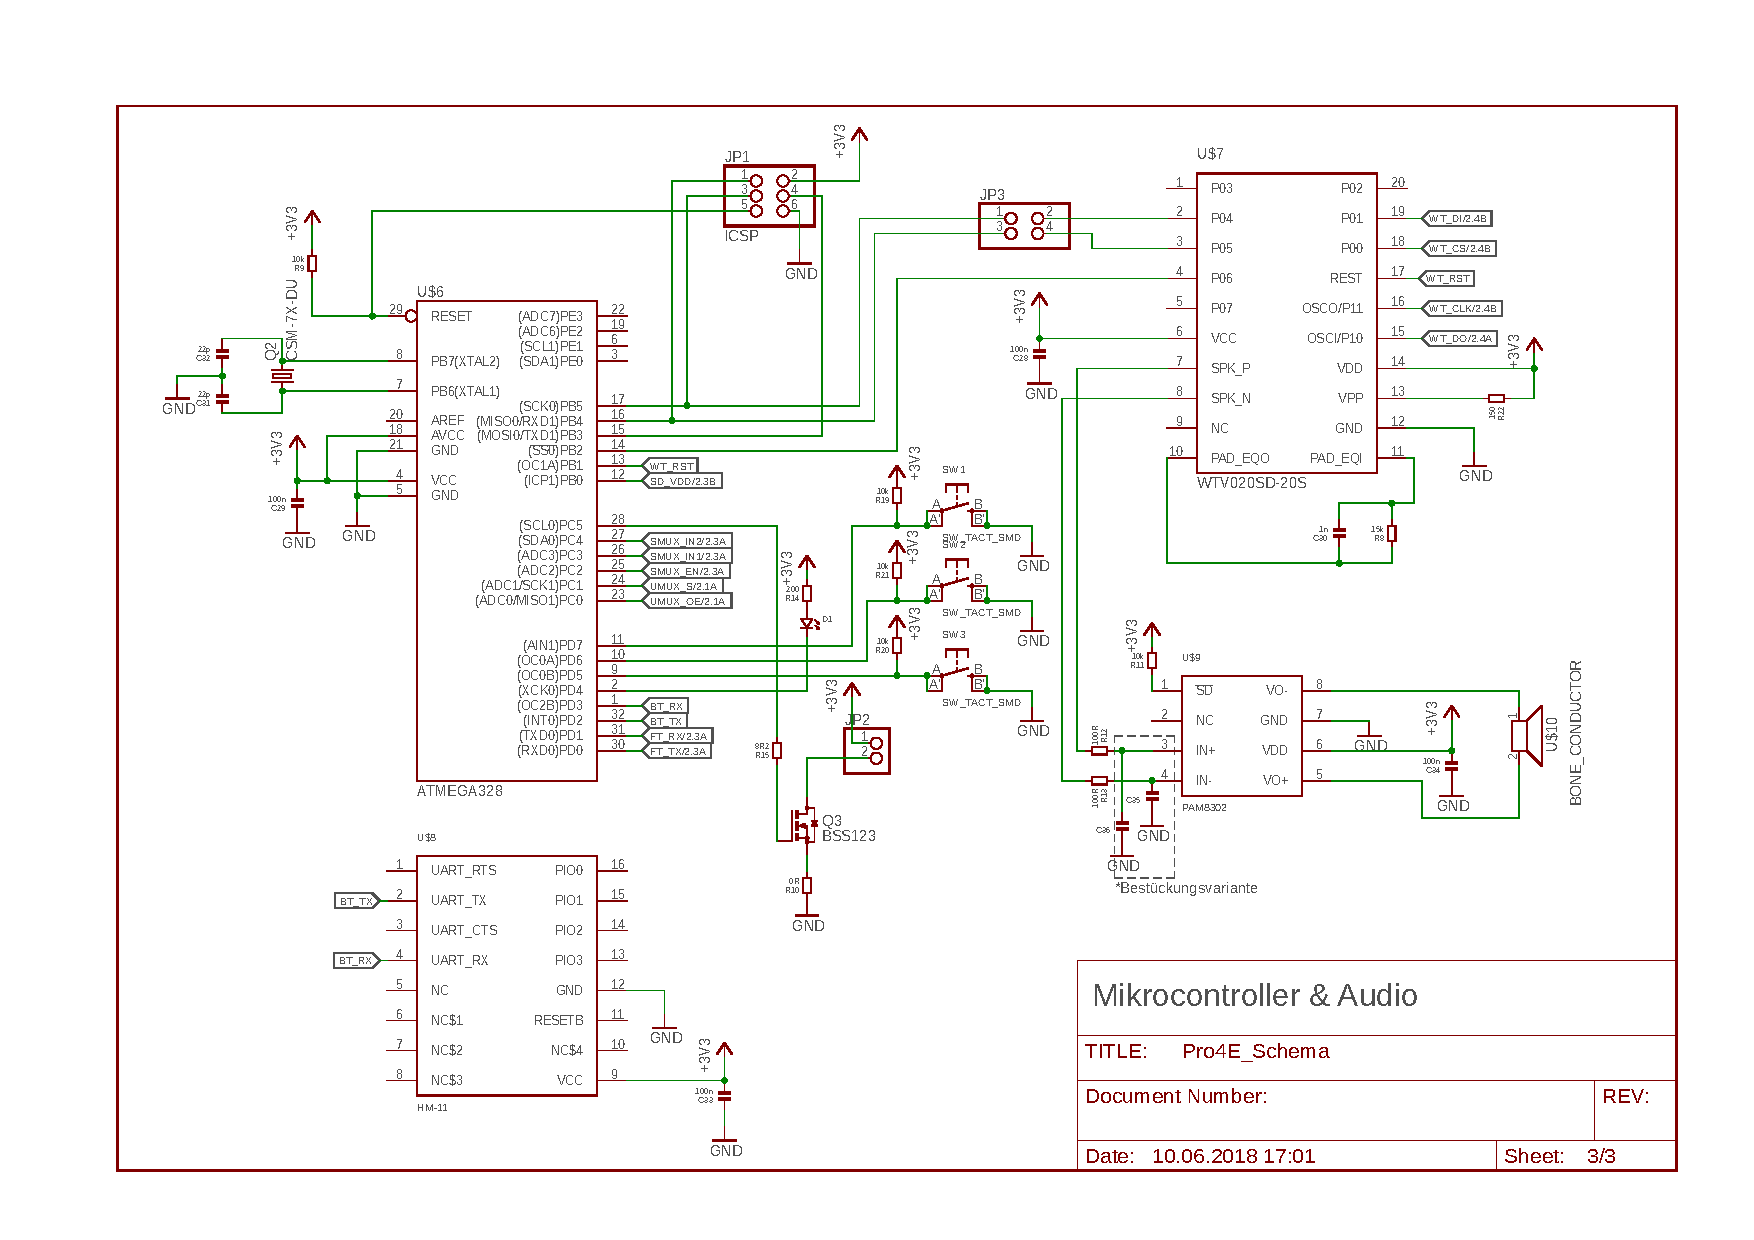
\includepdf[pages=1,fitpaper]{pdfs/Schema_Mikrocontroller}
\label{pdf:SchemaMikrocontroller}

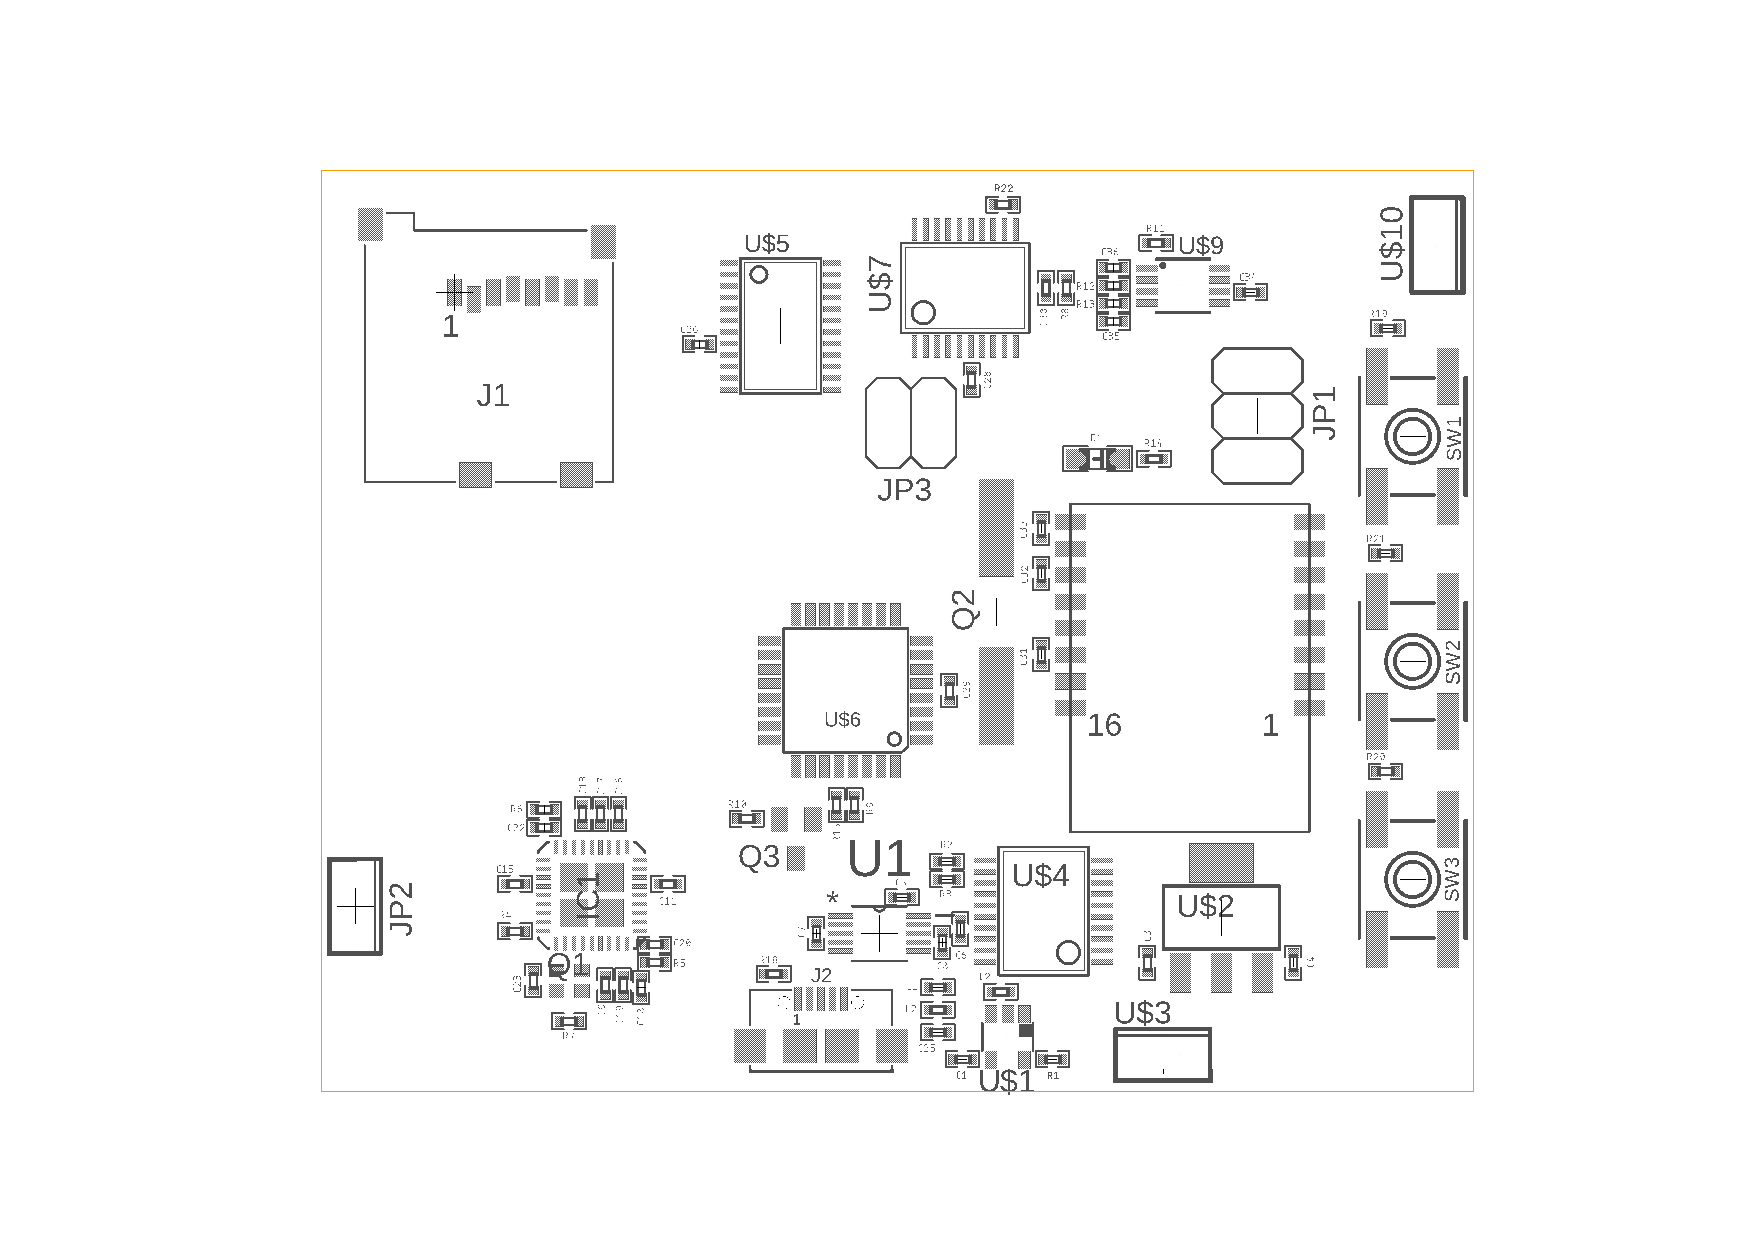
\includepdf[pages=1,fitpaper]{pdfs/Bestueckung_Top}
\label{pdf:BestueckungTop}

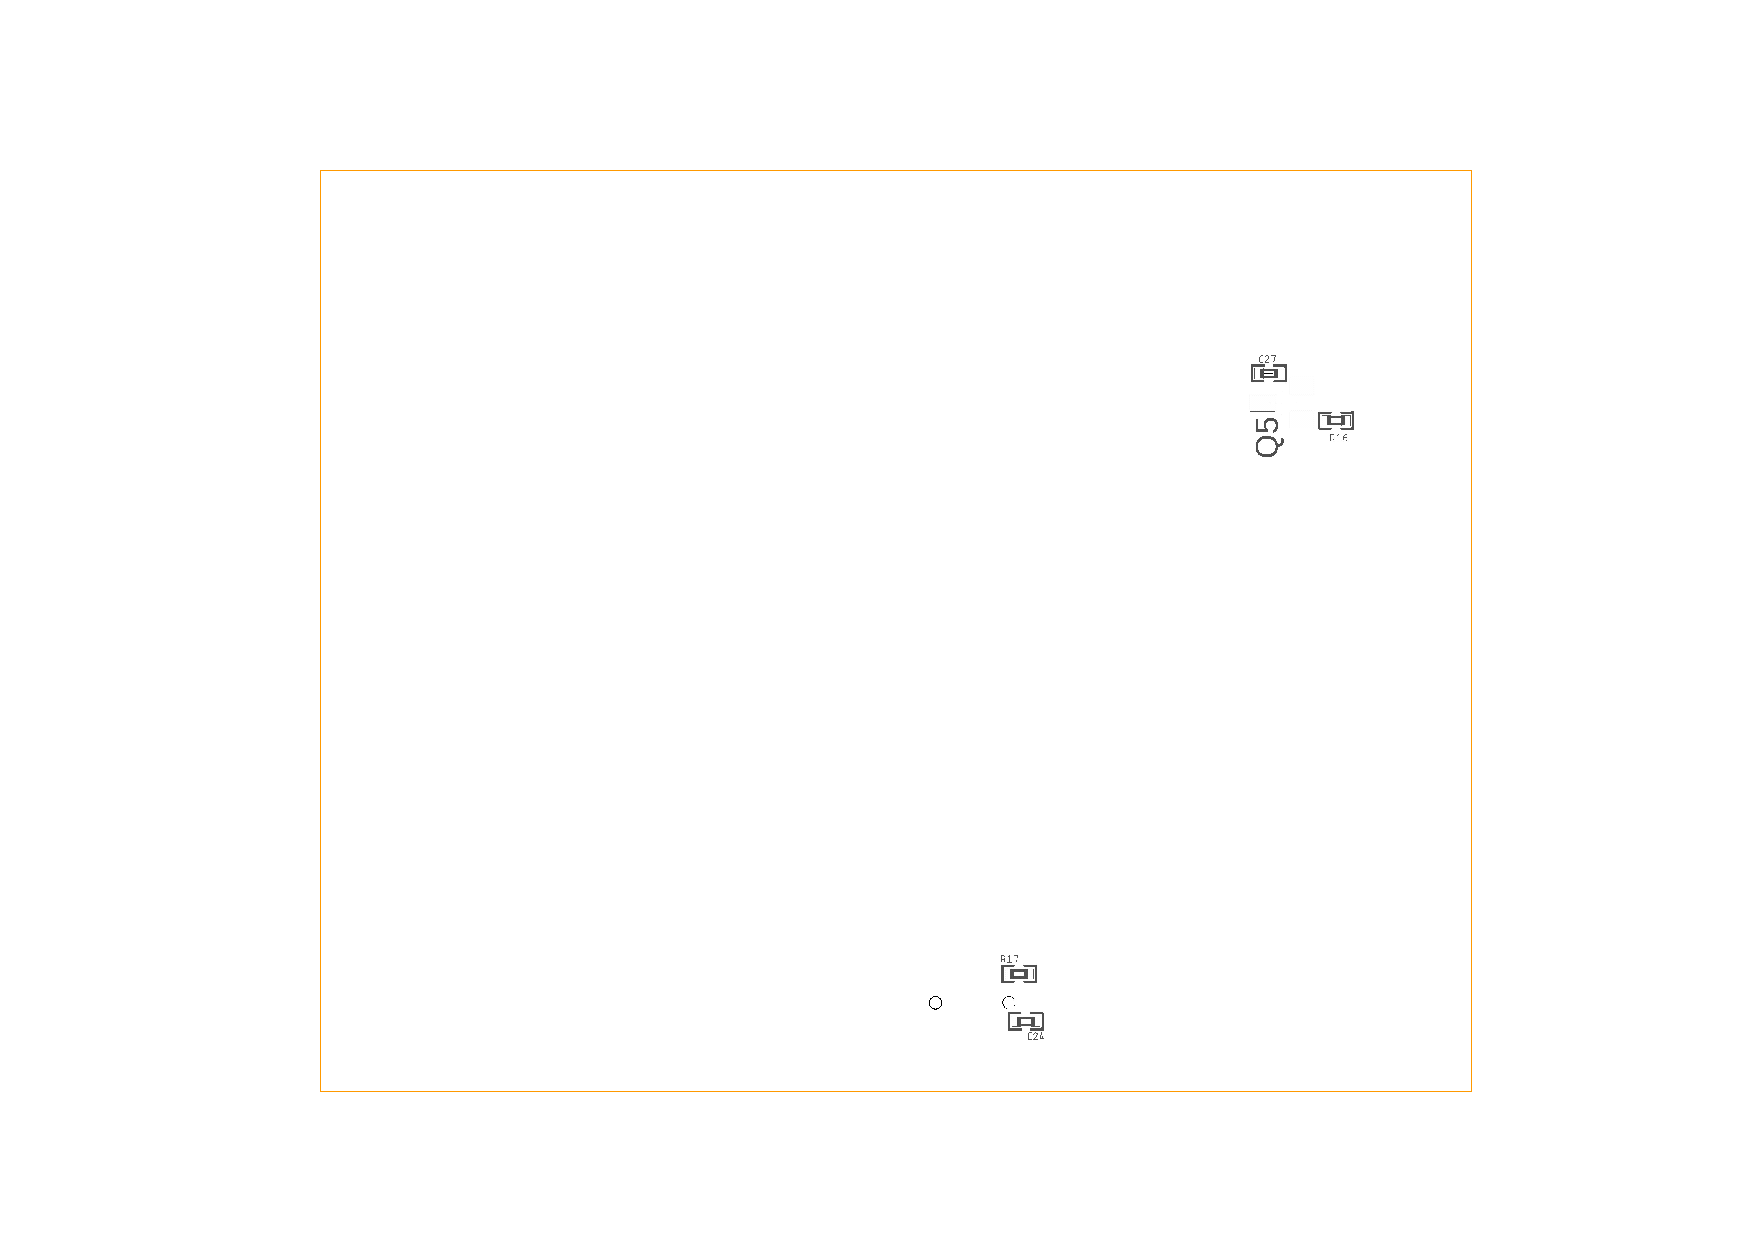
\includepdf[pages=1,fitpaper]{pdfs/Bestueckung_Bottom}
\label{pdf:BestueckungBottom}

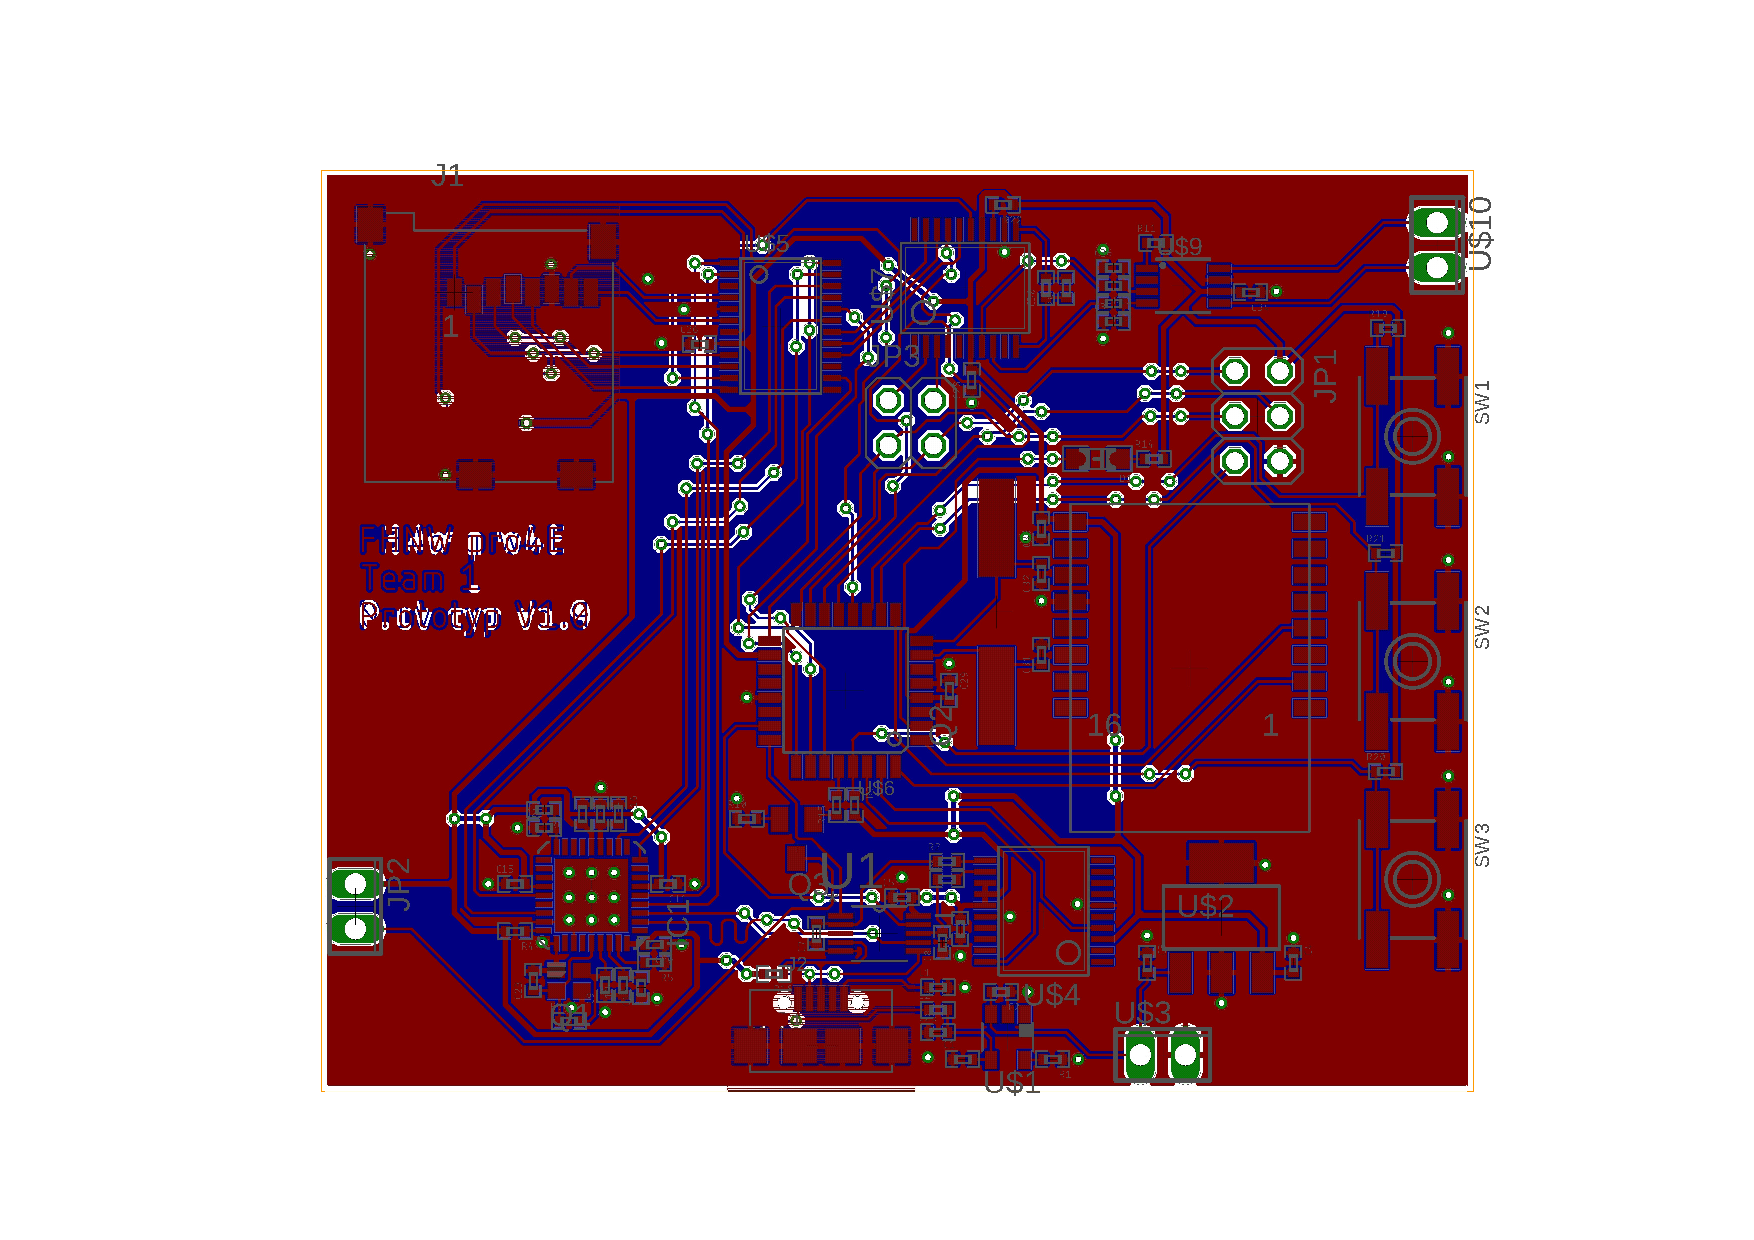
\includepdf[pages=1,fitpaper]{pdfs/Layout_all}
\label{pdf:LayoutAll}

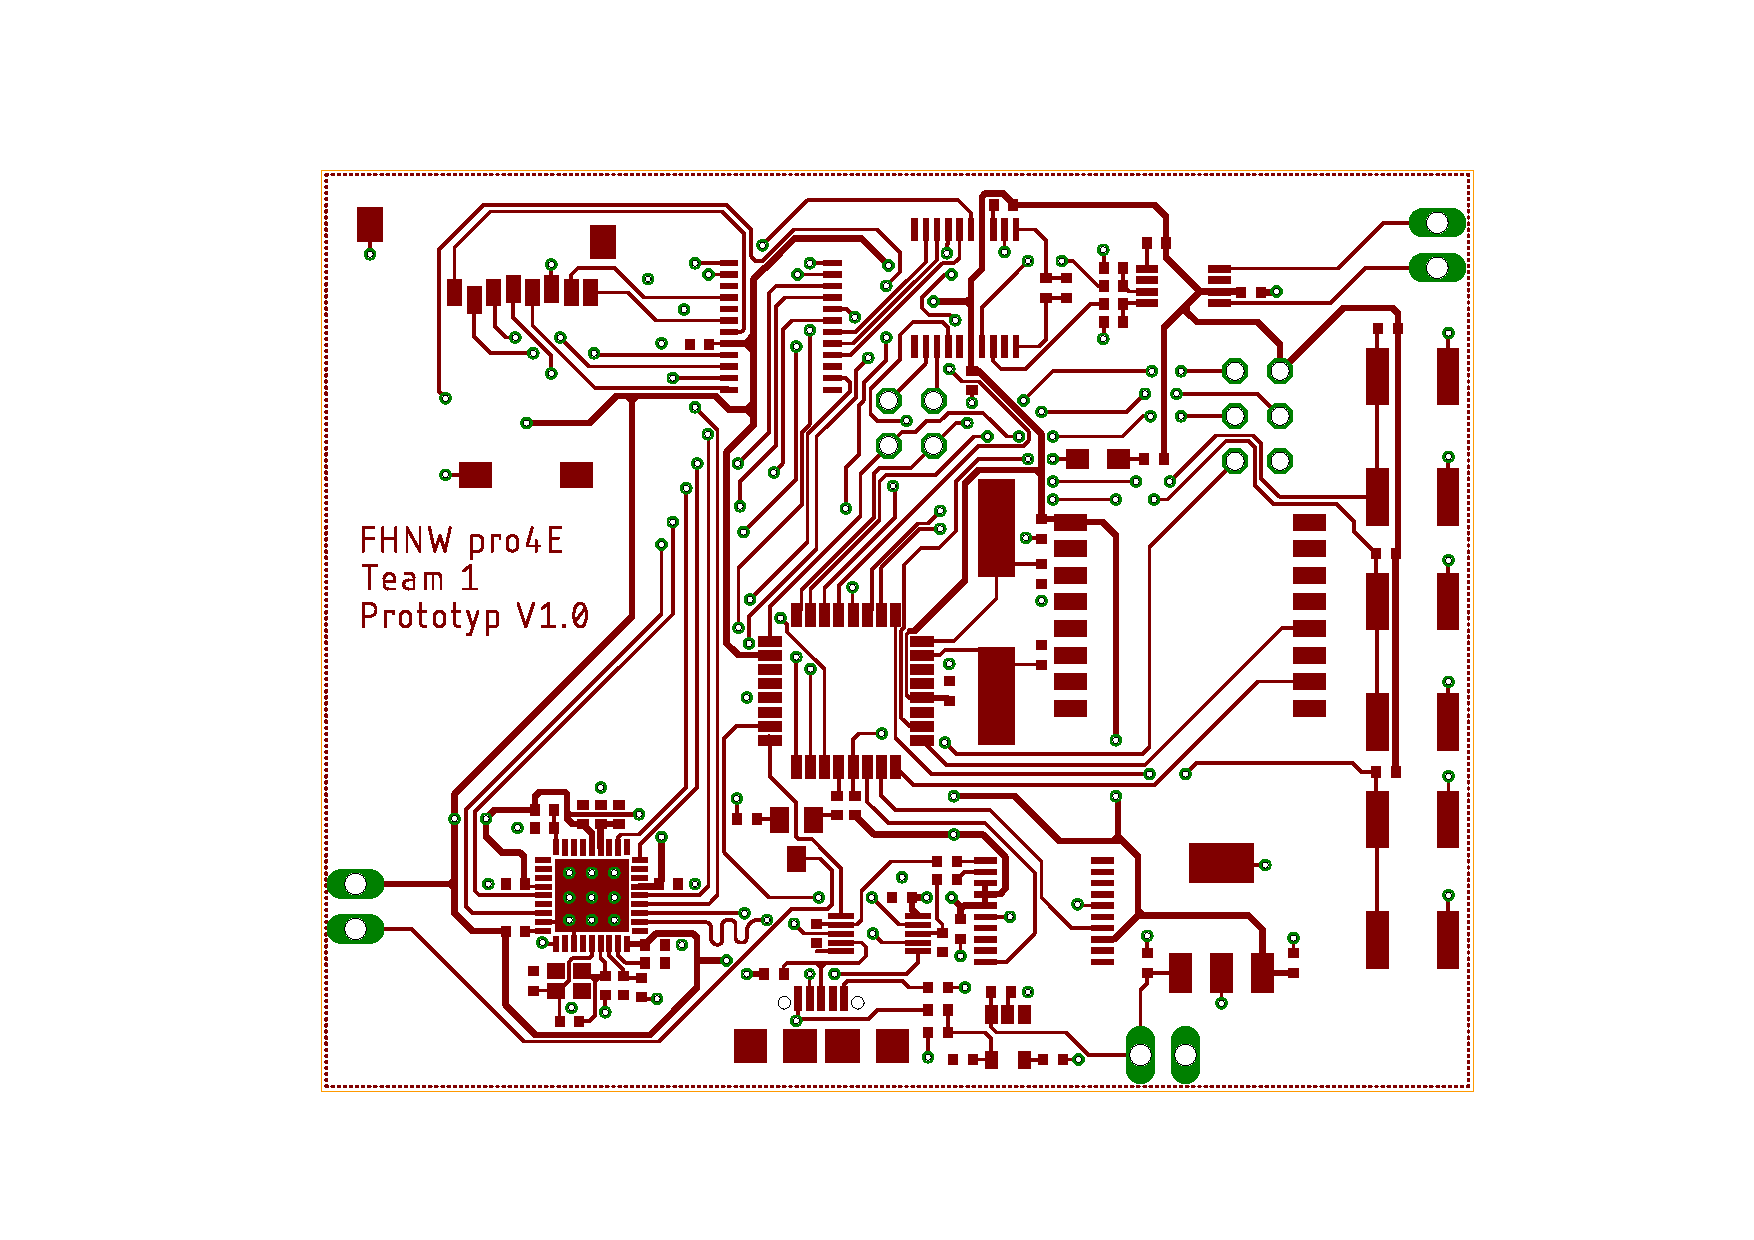
\includepdf[pages=1,fitpaper]{pdfs/Layout_top}
\label{pdf:LayoutTop}

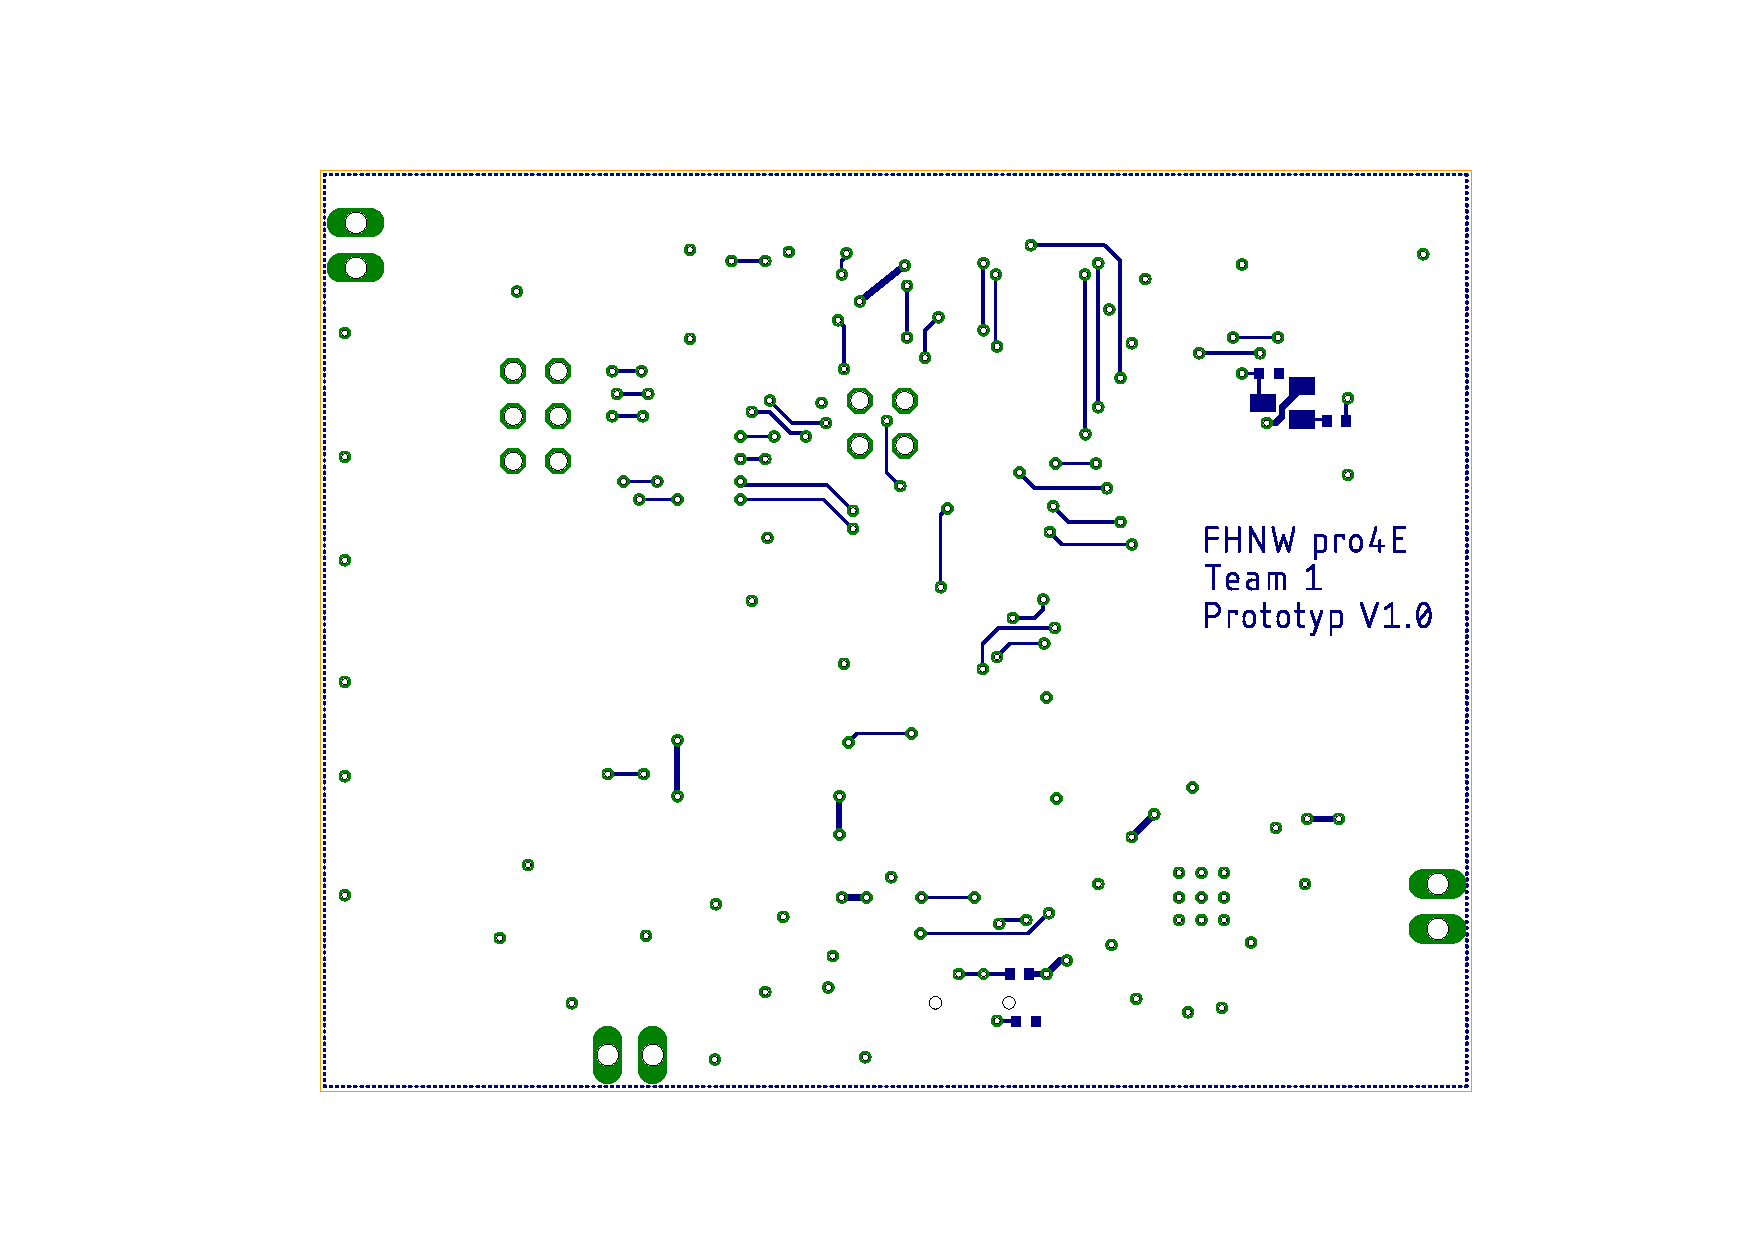
\includepdf[pages=1,fitpaper]{pdfs/Layout_bottom}
\label{pdf:LayoutBottom}


\end{document}


